\chapter{Dados de Ocorrência e Qualidade dos Registros}

\begin{chapteropening}
	
	Todo modelo de distribuição de espécies começa muito antes do ajuste de algoritmos estatísticos ou de técnicas de aprendizado de máquina. A qualidade de uma modelagem depende fundamentalmente da qualidade dos registros biológicos utilizados para representar a distribuição observada da espécie.
	
	Registros de ocorrência constituem evidências empíricas da presença de organismos em determinado local e momento. Esses registros são produzidos ao longo de décadas ou mesmo séculos por expedições científicas, inventários ecológicos, herbários, museus de história natural, programas de monitoramento e plataformas globais de compartilhamento de dados.
	
	Entretanto, registros biológicos não são observações perfeitas da realidade. Erros de identificação taxonômica, coordenadas incorretas, amostragens concentradas em áreas acessíveis e diferenças históricas no esforço de coleta podem introduzir vieses capazes de comprometer inferências ecológicas e projeções futuras.
	
	Nesta unidade, o leitor aprenderá como transformar registros brutos em uma base de dados robusta, coerente e adequada para Modelagem de Distribuição de Espécies. Utilizando \textit{Dinizia excelsa} como estudo de caso, serão apresentados os principais conceitos relacionados à obtenção, avaliação, limpeza, rarefação e preparação de dados de ocorrência para aplicações em conservação da biodiversidade e mudanças climáticas.
	
\end{chapteropening}

\begin{objetivos}
	
	Ao final desta unidade o estudante deverá ser capaz de:
	
	\begin{itemize}
		
		\item compreender o papel dos dados de ocorrência na Modelagem de Distribuição de Espécies;
		
		\item diferenciar os principais tipos de registros biológicos utilizados em estudos ecológicos;
		
		\item conhecer o funcionamento de herbários, museus e repositórios globais de biodiversidade;
		
		\item utilizar plataformas como GBIF, SpeciesLink e SiBBr;
		
		\item compreender conceitos de coordenadas geográficas, sistemas de referência e datum;
		
		\item identificar erros taxonômicos e geográficos em bases de ocorrência;
		
		\item reconhecer padrões de viés espacial e amostral;
		
		\item aplicar procedimentos de limpeza e controle de qualidade;
		
		\item compreender os fundamentos da rarefação espacial e do thinning;
		
		\item preparar uma base de registros adequada para modelagem de distribuição de espécies;
		
		\item interpretar o nicho climático ocupado por \textit{Dinizia excelsa};
		
		\item construir conjuntos de dados reproduzíveis para SDM.
		
	\end{itemize}
	
\end{objetivos}

\section{Dados de ocorrência como fundamento da SDM}

A distribuição geográfica das espécies constitui uma das questões centrais da Ecologia e da Biogeografia desde os trabalhos pioneiros de Grinnell, Elton e Hutchinson. Conforme discutido na Unidade 01, a ocorrência de uma espécie em determinado local resulta da interação entre condições ambientais, interações bióticas, processos históricos e limitações de dispersão. Entretanto, embora esses processos ecológicos operem continuamente na natureza, eles não são observados diretamente pelos pesquisadores. Em vez disso, o que efetivamente registramos são evidências pontuais da presença dos organismos em locais específicos. Essas observações constituem os chamados dados de ocorrência, que representam a principal fonte de informação utilizada em Modelagem de Distribuição de Espécies (Species Distribution Modelling – SDM) \parencite{grinnell1917field,hutchinson1957concluding,peterson2011ecological}.

Sob uma perspectiva ecológica, um registro de ocorrência pode ser entendido como uma amostra observada do nicho realizado de uma espécie. Cada ponto geográfico onde a espécie foi coletada, observada ou registrada corresponde a uma combinação particular de condições ambientais que permitiu sua persistência naquele local e naquele momento. Dessa forma, os registros de ocorrência funcionam como janelas empíricas através das quais os pesquisadores procuram inferir as relações entre organismos e ambiente. A lógica fundamental da SDM baseia-se justamente nesse princípio: utilizar padrões observados de ocorrência para identificar associações entre espécies e variáveis ambientais, permitindo estimar sua distribuição potencial em regiões não amostradas ou em cenários ambientais distintos \parencite{elith2009species,franklin2010mapping}.

Entretanto, é importante reconhecer que os registros disponíveis representam apenas uma fração da distribuição real das espécies. Em praticamente todos os ecossistemas do planeta, a probabilidade de uma espécie ser observada é influenciada não apenas por sua presença efetiva, mas também pela intensidade do esforço amostral, pela acessibilidade das áreas, pela experiência dos observadores e pela detectabilidade dos organismos. Consequentemente, a ausência de registros em determinada região não implica necessariamente ausência biológica. Muitas vezes, ela reflete simplesmente a inexistência de inventários ou dificuldades logísticas para a realização de amostragens. Esse problema é particularmente relevante em regiões tropicais, onde vastas áreas permanecem subamostradas mesmo após décadas de pesquisa científica \parencite{soberon2007grinnellian,guisan2017habitat}.

A distinção entre distribuição observada e distribuição real possui profundas implicações para a modelagem ecológica. Enquanto a distribuição observada corresponde ao conjunto de locais onde a espécie foi efetivamente registrada, a distribuição real inclui também áreas ambientalmente adequadas que ainda não foram amostradas ou onde a espécie não foi detectada. A função dos modelos de distribuição é justamente preencher essa lacuna de conhecimento, extrapolando as informações contidas nos registros disponíveis para estimar padrões mais amplos de adequabilidade ambiental. Nesse contexto, a qualidade dos modelos depende diretamente da capacidade dos dados de ocorrência representarem adequadamente a diversidade de condições ambientais utilizadas pela espécie \parencite{araujo2007ensemble,thuiller2019uncertainty}.

Do ponto de vista estatístico, os registros de ocorrência constituem a variável-resposta dos modelos correlativos de distribuição. Em algoritmos como GLM, GAM, Random Forest, Boosted Regression Trees e Maxent, cada ocorrência é associada aos valores ambientais extraídos para aquele local, formando a base empírica sobre a qual serão ajustadas as relações espécie-ambiente. Se os registros forem taxonomicamente incorretos, espacialmente imprecisos ou excessivamente concentrados em determinadas regiões, os modelos poderão aprender padrões artificiais que não refletem os processos ecológicos reais. Por essa razão, a obtenção e a preparação dos dados de ocorrência são frequentemente consideradas as etapas mais críticas de todo o fluxo de trabalho em SDM \parencite{elith2009species,franklin2010mapping}.

Nas últimas duas décadas, a disponibilidade de registros biológicos cresceu exponencialmente em decorrência da digitalização de herbários, museus e coleções científicas, bem como da criação de grandes infraestruturas globais de compartilhamento de dados sobre biodiversidade. Plataformas como o Global Biodiversity Information Facility (GBIF), o SpeciesLink e o Sistema de Informação sobre a Biodiversidade Brasileira (SiBBr) disponibilizam atualmente milhões de registros georreferenciados provenientes de diferentes instituições e períodos históricos. Essa revolução informacional ampliou significativamente as possibilidades de aplicação da SDM em escalas regionais e globais, permitindo análises de biodiversidade, planejamento sistemático da conservação, avaliação de invasões biológicas e projeções de impactos das mudanças climáticas \parencite{peterson2011ecological,guisan2017habitat}.

Contudo, o aumento da quantidade de dados não elimina a necessidade de avaliação crítica de sua qualidade. Registros provenientes de diferentes fontes frequentemente apresentam inconsistências taxonômicas, erros de georreferenciamento, duplicações, imprecisões temporais e vieses espaciais associados ao histórico de coleta. Em muitos casos, esses problemas podem produzir efeitos mais severos sobre os resultados dos modelos do que a própria escolha do algoritmo utilizado. Como consequência, estudos recentes enfatizam que a curadoria dos dados de ocorrência deve ser tratada como uma etapa científica fundamental, e não apenas como um procedimento técnico preliminar \parencite{zurell2020standard,zizka2019coordinatecleaner}.

A importância dos dados de ocorrência torna-se ainda mais evidente quando consideramos aplicações voltadas à conservação da biodiversidade e às mudanças climáticas. Projeções futuras de distribuição dependem inteiramente das relações ecológicas inferidas a partir dos registros atuais. Caso os dados utilizados sejam enviesados ou inadequados, as previsões resultantes poderão indicar áreas prioritárias incorretas para conservação, subestimar riscos de extinção ou superestimar a capacidade de persistência das espécies em cenários climáticos futuros. Em outras palavras, a robustez de qualquer inferência biogeográfica é limitada pela qualidade das observações que a sustentam \parencite{araujo2019standards,franklin2010mapping}.

Ao longo desta unidade, veremos que transformar registros brutos em uma base de dados adequada para modelagem envolve uma série de etapas interdependentes, incluindo validação taxonômica, verificação geográfica, remoção de duplicatas, controle de qualidade, avaliação de vieses espaciais, rarefação amostral e extração de informações ambientais. Esses procedimentos não apenas aumentam a confiabilidade dos modelos, mas também aproximam os dados observados dos processos ecológicos que buscamos compreender. Assim, antes mesmo de discutir algoritmos de modelagem, é essencial compreender que a qualidade de uma SDM começa pela qualidade de seus registros de ocorrência.

\section{O que é um registro biológico?}

Os dados de ocorrência utilizados em Modelagem de Distribuição de Espécies são derivados de registros biológicos produzidos por diferentes atividades de pesquisa, monitoramento e documentação da biodiversidade. Embora frequentemente representados apenas como pontos em um mapa, esses registros constituem evidências científicas que documentam a presença de organismos em determinado local e momento. Cada registro carrega consigo um conjunto de informações associadas à observação da espécie, incluindo sua identidade taxonômica, localização geográfica, data de coleta e, em muitos casos, detalhes sobre o ambiente e os métodos utilizados para sua obtenção \parencite{franklin2010mapping,peterson2011ecological}.

Historicamente, a principal forma de registro biológico foi a coleta de espécimes testemunho, também conhecidos como vouchers biológicos. Nesse procedimento, um exemplar do organismo é coletado, preservado e depositado em uma coleção científica, tornando-se uma evidência física permanente da ocorrência da espécie. A existência do voucher permite futuras revisões taxonômicas, reidentificações e validações independentes, conferindo elevada confiabilidade aos dados produzidos. Por essa razão, espécimes testemunho continuam sendo considerados o padrão-ouro para documentação da biodiversidade \parencite{funk2018collections}.

Nem todos os registros biológicos, entretanto, dependem da coleta física de organismos. Observações diretas em campo constituem uma importante fonte de informação, especialmente para grupos nos quais a coleta é difícil, inviável ou eticamente restrita. Avanços tecnológicos ampliaram significativamente a utilização de registros observacionais, incluindo fotografias georreferenciadas, gravações acústicas, imagens obtidas por armadilhas fotográficas e registros realizados por aplicativos móveis. Embora possam apresentar níveis variáveis de confiabilidade taxonômica, essas observações aumentam substancialmente a cobertura espacial e temporal dos bancos de dados de biodiversidade \parencite{guisan2017habitat}.

Outra importante fonte de dados de ocorrência são os inventários ecológicos e florestais. Esses estudos geralmente seguem protocolos padronizados de amostragem e produzem informações detalhadas sobre composição florística, abundância, estrutura populacional e características ambientais. Em regiões tropicais, inventários florestais têm desempenhado papel fundamental na ampliação do conhecimento sobre a distribuição de espécies arbóreas, especialmente em áreas remotas onde os registros provenientes de herbários ainda são escassos \parencite{phillips2019rainfor}.

Entre os inventários ecológicos, destacam-se as parcelas permanentes de monitoramento. Diferentemente de levantamentos pontuais, essas parcelas são revisitadas periodicamente ao longo de anos ou décadas, permitindo acompanhar processos ecológicos dinâmicos, como crescimento, mortalidade, recrutamento e mudanças na composição das comunidades. Redes internacionais de monitoramento, como RAINFOR e ForestPlots, constituem atualmente algumas das mais importantes fontes de dados sobre a distribuição e a dinâmica das florestas tropicais do planeta \parencite{malhi2002rainfor,lopezgonzalez2011forestplots}.

Nos últimos anos, sensores automáticos passaram a gerar novas formas de registros biológicos. Armadilhas fotográficas, sensores acústicos, radares biológicos, drones e sistemas automatizados de monitoramento ambiental permitem registrar organismos continuamente, muitas vezes em locais de difícil acesso. Esses métodos ampliam a capacidade de detecção de espécies e reduzem parte dos vieses associados à observação humana, embora também introduzam novos desafios relacionados ao armazenamento, processamento e interpretação de grandes volumes de dados \parencite{burton2015wildlife}.

Paralelamente, a expansão da ciência cidadã transformou profundamente a produção de dados sobre biodiversidade em escala global. Plataformas colaborativas permitem que observadores não especialistas contribuam com registros georreferenciados de espécies, frequentemente acompanhados por fotografias e informações complementares. Embora a qualidade taxonômica desses registros possa variar, mecanismos de validação comunitária têm demonstrado elevado potencial para geração de dados úteis em estudos ecológicos e biogeográficos. Atualmente, milhões de registros disponibilizados por iniciativas de ciência cidadã são incorporados rotineiramente a análises de distribuição de espécies e monitoramento da biodiversidade \parencite{sullivan2014ebird,callaghan2021global}.

Independentemente de sua origem, todos os registros biológicos compartilham uma característica fundamental: representam observações parciais da distribuição das espécies. Consequentemente, compreender a natureza, as vantagens e as limitações de cada tipo de registro é essencial para avaliar sua adequação a diferentes aplicações em Modelagem de Distribuição de Espécies.

\begin{table}[H]
	\centering
	\caption{Principais tipos de registros biológicos utilizados em estudos de distribuição de espécies.}
	\label{tab:tipos_registros}
	\begin{tabular}{p{3.5cm}p{5.5cm}p{5.5cm}}
		\toprule
		\textbf{Tipo de registro} &
		\textbf{Vantagens} &
		\textbf{Limitações} \\
		\midrule
		
		Espécime testemunho (voucher)
		&
		Alta confiabilidade taxonômica; possibilidade de reidentificação; documentação permanente.
		&
		Coleta mais custosa; cobertura espacial frequentemente limitada.
		
		\\
		
		Observação de campo
		&
		Grande quantidade de registros; rápida obtenção de dados.
		&
		Possibilidade de erros de identificação.
		
		\\
		
		Inventários ecológicos
		&
		Protocolos padronizados; informações ambientais detalhadas.
		&
		Cobertura espacial geralmente restrita.
		
		\\
		
		Parcelas permanentes
		&
		Monitoramento de longo prazo; dados ecológicos robustos.
		&
		Baixa representatividade espacial em escala continental.
		
		\\
		
		Sensores automáticos
		&
		Monitoramento contínuo; elevada detectabilidade.
		&
		Grande volume de dados e necessidade de processamento especializado.
		
		\\
		
		Ciência cidadã
		&
		Cobertura espacial ampla; rápida expansão de registros.
		&
		Qualidade taxonômica variável e viés de amostragem.
		
		\\
		\bottomrule
	\end{tabular}
\end{table}

\section{Herbários, museus e coleções biológicas}

Muito antes do surgimento dos bancos de dados digitais e das plataformas globais de biodiversidade, o conhecimento sobre a distribuição das espécies era construído a partir das coleções biológicas. Herbários, museus de história natural e coleções zoológicas desempenharam papel central no desenvolvimento da Taxonomia, da Biogeografia e da Ecologia, preservando evidências materiais da biodiversidade coletadas ao longo de séculos de exploração científica \parencite{suarez2004value}.

Nas ciências botânicas, os herbários constituem os principais repositórios de informações sobre a ocorrência de espécies vegetais. Um herbário é uma coleção organizada de plantas prensadas, secas e armazenadas segundo protocolos padronizados, acompanhadas por informações detalhadas sobre local de coleta, data, ambiente, coletor e identificação taxonômica. Muitos dos registros utilizados atualmente em estudos de Modelagem de Distribuição de Espécies foram originalmente produzidos por expedições botânicas realizadas décadas ou mesmo séculos atrás \parencite{funk2018collections}.

O elemento central de uma coleção biológica é o chamado voucher ou espécime testemunho. O voucher representa a evidência física que comprova a ocorrência de determinada espécie em um local específico. Diferentemente de uma simples observação, o voucher pode ser reexaminado por especialistas, permitindo corrigir erros taxonômicos, atualizar nomenclaturas e incorporar novos conhecimentos sistemáticos. Em um contexto de mudanças constantes na classificação biológica, essa possibilidade de verificação independente torna os vouchers instrumentos fundamentais para garantir a confiabilidade dos registros utilizados em pesquisas ecológicas e biogeográficas.

Além de preservar espécimes, as coleções biológicas desempenham importante função de curadoria científica. Curadores e taxonomistas são responsáveis pela organização, manutenção, atualização nomenclatural e validação dos exemplares depositados. Esse trabalho contínuo reduz inconsistências taxonômicas e assegura que as informações associadas aos espécimes permaneçam úteis para futuras gerações de pesquisadores \parencite{pyke2010biological}.

Nas últimas décadas, a digitalização das coleções revolucionou o acesso às informações sobre biodiversidade. Milhões de espécimes foram convertidos em registros digitais contendo imagens de alta resolução, coordenadas geográficas e metadados padronizados. Como resultado, informações anteriormente restritas a instituições específicas passaram a integrar grandes redes internacionais de compartilhamento de dados, ampliando enormemente sua utilização em estudos ecológicos, biogeográficos e conservacionistas \parencite{nelson2015digitization}.

Para a Modelagem de Distribuição de Espécies, herbários e museus representam muito mais do que simples depósitos de espécimes. Eles constituem verdadeiras bibliotecas da biodiversidade, preservando registros históricos que permitem reconstruir distribuições passadas, avaliar mudanças temporais e compreender padrões ecológicos em múltiplas escalas espaciais.

```

\begin{conceito}[title={\faBook\quad O papel do voucher em estudos de SDM}]
	O voucher biológico constitui a evidência física que sustenta a validade de um registro de ocorrência. Em Modelagem de Distribuição de Espécies, registros associados a espécimes testemunho apresentam maior confiabilidade taxonômica e permitem verificações independentes futuras, reduzindo incertezas relacionadas à identificação das espécies.
\end{conceito}

\section{Infraestrutura global de dados sobre biodiversidade}

A digitalização das coleções biológicas e a expansão da internet transformaram profundamente a forma como dados sobre biodiversidade são armazenados, compartilhados e utilizados. Atualmente, pesquisadores podem acessar milhões de registros de ocorrência provenientes de milhares de instituições distribuídas ao redor do mundo. Essa infraestrutura global de informação constitui um dos principais pilares da pesquisa moderna em Biogeografia, Conservação e Modelagem de Distribuição de Espécies \parencite{edwards2000gbif}.

A principal iniciativa internacional nesse contexto é o Global Biodiversity Information Facility (GBIF). Criado em 2001, o GBIF integra dados provenientes de herbários, museus, universidades, programas de monitoramento e projetos de ciência cidadã, disponibilizando gratuitamente centenas de milhões de registros de ocorrência em escala global. Devido à sua abrangência taxonômica e geográfica, o GBIF tornou-se a principal fonte de dados para estudos de SDM em múltiplas escalas espaciais \parencite{gbif2024}.

Na América Latina, uma das iniciativas mais importantes é o SpeciesLink, desenvolvido pelo Centro de Referência em Informação Ambiental (CRIA). A plataforma integra informações provenientes de centenas de coleções biológicas brasileiras e latino-americanas, oferecendo acesso a registros detalhados e frequentemente mais atualizados para espécies neotropicais. Em muitos casos, o SpeciesLink disponibiliza informações complementares que ainda não foram incorporadas ao GBIF.

Complementando essas iniciativas, o Sistema de Informação sobre a Biodiversidade Brasileira (SiBBr) atua como infraestrutura nacional de integração e disponibilização de dados sobre biodiversidade no Brasil. O SiBBr promove a padronização de informações biológicas e facilita a interoperabilidade entre diferentes bancos de dados nacionais e internacionais.

Além das bases tradicionais derivadas de coleções científicas, plataformas de ciência cidadã passaram a desempenhar papel crescente na geração de registros biológicos. O iNaturalist destaca-se como uma das iniciativas mais bem-sucedidas nesse contexto, permitindo que observadores registrem organismos por meio de fotografias georreferenciadas submetidas à validação colaborativa da comunidade científica e de usuários especializados.

No contexto das florestas tropicais, bases de dados derivadas de parcelas permanentes assumem importância estratégica. Redes como ForestPlots e RAINFOR reúnem informações provenientes de centenas de parcelas distribuídas pela Amazônia, África e Ásia tropical, fornecendo dados de alta qualidade sobre composição florística, estrutura florestal e dinâmica ecológica. Embora seu objetivo principal não seja a documentação de ocorrências individuais, esses bancos de dados constituem fontes extremamente valiosas para estudos envolvendo espécies arbóreas tropicais, incluindo aplicações em SDM.

A existência dessa infraestrutura global representa uma das maiores revoluções da ciência da biodiversidade nas últimas décadas. Entretanto, a facilidade de acesso aos dados não elimina a necessidade de avaliação crítica de sua qualidade. Como veremos nas próximas seções, registros obtidos em diferentes plataformas podem apresentar inconsistências taxonômicas, erros geográficos e vieses amostrais que precisam ser cuidadosamente tratados antes de sua utilização em modelos ecológicos.

\begin{table}[H]
	\centering
	\caption{Principais infraestruturas de dados utilizadas em estudos de distribuição de espécies.}
	\label{tab:bases_biodiversidade}
	\begin{tabular}{p{3cm}p{4cm}p{3cm}p{4cm}}
		\toprule
		\textbf{Plataforma} &
		\textbf{Escala} &
		\textbf{Tipo principal de dado} &
		\textbf{Aplicação em SDM} \\
		\midrule
		
		GBIF &
		Global &
		Ocorrências biológicas &
		Fonte principal de registros.
		
		\\
		
		SpeciesLink &
		Brasil e América Latina &
		Coleções biológicas &
		Espécies neotropicais.
		
		\\
		
		SiBBr &
		Brasil &
		Dados integrados de biodiversidade &
		Complementação de registros nacionais.
		
		\\
		
		iNaturalist &
		Global &
		Ciência cidadã &
		Ampliação da cobertura espacial.
		
		\\
		
		ForestPlots &
		Florestas tropicais &
		Parcelas permanentes &
		Distribuição e ecologia de árvores.
		
		\\
		
		RAINFOR &
		Amazônia &
		Parcelas permanentes &
		Monitoramento de espécies arbóreas.
		
		\\
		\bottomrule
	\end{tabular}
\end{table}

\section{Estrutura de um registro de ocorrência}

Independentemente da fonte de origem, todo registro de ocorrência é composto por um conjunto mínimo de informações que documentam a presença de uma espécie em determinado local e momento. Em Modelagem de Distribuição de Espécies, esses atributos são fundamentais porque permitem associar observações biológicas às condições ambientais existentes na área de ocorrência \parencite{peterson2011ecological,franklin2010mapping}.

O elemento central de qualquer registro é a identificação taxonômica da espécie. O nome científico constitui a ligação entre a observação realizada em campo e todo o conhecimento acumulado sobre aquele organismo. Erros de identificação, sinonímias ou nomenclaturas desatualizadas podem gerar inconsistências que se propagam para as etapas posteriores da modelagem, tornando indispensável a padronização taxonômica dos registros antes de qualquer análise \parencite{guisan2017habitat}.

Além da identificação da espécie, registros de ocorrência geralmente incluem coordenadas geográficas representadas por latitude e longitude. Essas informações permitem localizar espacialmente o organismo e associar cada ocorrência a variáveis ambientais derivadas de mapas climáticos, topográficos ou edáficos. Em estudos de SDM, as coordenadas constituem a ponte entre os dados biológicos e o ambiente utilizado pelos modelos \parencite{elith2009species}.

Outro atributo importante é a data de coleta ou observação. Informações temporais permitem avaliar a atualidade dos registros e identificar possíveis mudanças na distribuição das espécies ao longo do tempo. Embora muitos modelos utilizem conjuntamente registros obtidos em diferentes períodos, a avaliação temporal dos dados representa uma etapa importante do controle de qualidade \parencite{franklin2010mapping}.

Os registros também costumam conter informações sobre o coletor, observador ou instituição responsável pela documentação da ocorrência. Esses metadados permitem rastrear a origem da informação, verificar sua confiabilidade e, quando necessário, consultar a fonte original do registro.

Por fim, muitos bancos de dados disponibilizam estimativas de precisão espacial ou incerteza geográfica. Esse atributo indica o grau de confiança associado às coordenadas registradas e auxilia na identificação de ocorrências potencialmente problemáticas. Registros com baixa precisão espacial podem comprometer a extração de variáveis ambientais e introduzir erros nos modelos de distribuição \parencite{zizka2019coordinatecleaner}.

Embora diferentes plataformas utilizem estruturas de dados específicas, a maioria dos registros atualmente segue padrões internacionais de compartilhamento de informações sobre biodiversidade, permitindo a integração de dados provenientes de múltiplas fontes. Essa padronização é um dos fatores que possibilita a construção de bases de ocorrência em escala regional, continental e global.

\begin{table}[H]
	\centering
	\caption{Exemplo simplificado de um registro de ocorrência utilizado em SDM.}
	\label{tab:registro_ocorrencia}
	\begin{tabular}{ll}
		\toprule
		\textbf{Campo} & \textbf{Valor exemplo} \\
		\midrule
		Espécie & \textit{Dinizia excelsa} \\
		Latitude & 1.2456 \\
		Longitude & -52.3187 \\
		Data & 2018-07-14 \\
		Coletor & R. B. Lima \\
		Instituição & Herbário IAN \\
		Precisão espacial & 30 m \\
		Fonte & GBIF \\
		\bottomrule
	\end{tabular}
\end{table}

\section{Coordenadas geográficas e georreferenciamento}

A localização espacial dos organismos constitui um dos componentes centrais da Modelagem de Distribuição de Espécies. Em estudos de SDM, cada registro de ocorrência precisa ser associado a uma posição geográfica específica para que as condições ambientais presentes naquele local possam ser caracterizadas e utilizadas na construção dos modelos. Dessa forma, compreender os fundamentos do georreferenciamento é um passo essencial para garantir a qualidade das análises ecológicas e biogeográficas \parencite{franklin2010mapping}.

A forma mais comum de representar a localização de um organismo é por meio de coordenadas geográficas expressas em latitude e longitude. A latitude indica a posição ao norte ou ao sul da Linha do Equador, enquanto a longitude representa a posição a leste ou oeste do Meridiano de Greenwich. Juntas, essas duas coordenadas permitem localizar qualquer ponto na superfície terrestre com elevada precisão.

Entretanto, coordenadas geográficas não possuem significado isoladamente. Sua interpretação depende de um sistema de referência geodésico, também denominado datum. O datum define matematicamente a forma e o tamanho da Terra utilizados para representar posições geográficas. Atualmente, o sistema mais utilizado em bancos de dados de biodiversidade é o World Geodetic System 1984 (WGS84), adotado por sistemas GPS, plataformas de biodiversidade e grande parte dos produtos cartográficos globais \parencite{hijmans2021species}.

Além dos sistemas de coordenadas geográficas, diversas aplicações utilizam projeções cartográficas para representar a superfície curva da Terra em mapas planos. Embora projeções sejam indispensáveis para análises espaciais e cálculos de distância, área e direção, elas também podem introduzir distorções se utilizadas inadequadamente. Por essa razão, é fundamental que todos os dados espaciais empregados em um estudo estejam compatíveis em relação ao sistema de referência adotado.

Erros associados à conversão de coordenadas constituem uma das causas mais frequentes de problemas em bases de ocorrência. Diferenças entre datums, inversões de sinais, erros de digitação e transformações incorretas entre sistemas de projeção podem deslocar registros por centenas ou até milhares de quilômetros. Em consequência, pontos biologicamente plausíveis podem ser erroneamente posicionados em ambientes completamente distintos daqueles efetivamente ocupados pela espécie \parencite{zizka2019coordinatecleaner}.

Embora os sistemas modernos de posicionamento tenham reduzido significativamente esse tipo de problema, a verificação das coordenadas continua sendo uma etapa indispensável do controle de qualidade em estudos de Modelagem de Distribuição de Espécies. Antes mesmo de avaliar aspectos ecológicos dos registros, é necessário assegurar que cada ocorrência esteja corretamente localizada no espaço geográfico.

\section{Principais erros em dados de ocorrência}

A crescente disponibilidade de registros biológicos em plataformas digitais representa uma das maiores conquistas da ciência da biodiversidade. Entretanto, a ampliação do volume de dados não garante automaticamente sua qualidade. Registros provenientes de diferentes instituições, períodos históricos e metodologias de coleta frequentemente apresentam inconsistências que podem comprometer análises ecológicas e modelos de distribuição. Por essa razão, a identificação e correção de erros constituem uma etapa fundamental da preparação dos dados \parencite{peterson2011ecological,zizka2019coordinatecleaner}.

\subsection{Erros taxonômicos}

Os erros taxonômicos estão entre os problemas mais comuns encontrados em bases de ocorrência. Mudanças nomenclaturais ao longo do tempo podem fazer com que uma mesma espécie apareça registrada sob diferentes nomes científicos. Além disso, erros de grafia, abreviações inconsistentes e atualizações taxonômicas incompletas podem gerar duplicações artificiais ou fragmentação dos registros.

Outro problema frequente ocorre quando espécies morfologicamente semelhantes são confundidas durante a identificação. Em grupos taxonomicamente complexos, registros incorretamente identificados podem expandir artificialmente a distribuição conhecida da espécie ou associá-la a condições ambientais inadequadas. Consequentemente, a validação taxonômica deve preceder qualquer análise espacial ou ecológica \parencite{guisan2017habitat}.

\subsection{Erros geográficos}

Os erros geográficos referem-se a inconsistências associadas às coordenadas dos registros. Entre os exemplos mais comuns estão pontos localizados em oceanos, coordenadas incompatíveis com a distribuição conhecida da espécie, inversões de latitude e longitude e erros de sinal associados aos hemisférios Norte-Sul ou Leste-Oeste.

Em muitos casos, pequenos erros de digitação podem deslocar registros para milhares de quilômetros de distância de sua localização original. Como os modelos utilizam as condições ambientais extraídas desses pontos, registros geograficamente incorretos podem gerar relações ecológicas artificiais e comprometer a qualidade das predições \parencite{franklin2010mapping}.

\subsection{Registros institucionais}

Um padrão recorrente em bancos de dados de biodiversidade é a presença de registros associados à localização das instituições responsáveis pela curadoria dos espécimes. Quando a localidade original de coleta não é conhecida, coordenadas podem ser atribuídas à sede do herbário, museu ou universidade onde o material foi depositado.

Esse problema produz concentrações artificiais de registros em capitais, centros urbanos ou instituições científicas. Como tais pontos não representam locais reais de ocorrência da espécie, sua utilização em SDM pode introduzir vieses importantes nas análises \parencite{zizka2019coordinatecleaner}.

\subsection{Registros \textit{ex situ}}

Nem todos os organismos registrados em bancos de dados encontram-se em populações naturais. Jardins botânicos, arboretos, coleções vivas e plantios experimentais frequentemente contêm indivíduos cultivados fora de sua área de distribuição natural.

Embora esses registros possuam valor científico para diversos estudos, eles normalmente não devem ser utilizados em Modelagem de Distribuição de Espécies, pois refletem a ação humana e não necessariamente as condições ecológicas que limitam a ocorrência natural da espécie. A identificação e remoção desses registros representam uma etapa importante do controle de qualidade.

Atualmente, diversos procedimentos de limpeza podem ser automatizados por ferramentas computacionais especializadas. Entre elas, destaca-se o pacote \texttt{CoordinateCleaner}, amplamente utilizado para detectar registros localizados em capitais, instituições científicas, centros populacionais, coordenadas duplicadas, pontos no oceano e outras anomalias espaciais. Essas ferramentas não substituem a avaliação crítica dos dados, mas aumentam significativamente a eficiência do processo de curadoria \parencite{zizka2019coordinatecleaner}.

\section{Viés amostral e viés espacial}

Mesmo quando os registros apresentam identificação taxonômica correta e coordenadas geograficamente válidas, eles raramente representam uma amostra aleatória da distribuição das espécies. Em praticamente todos os programas de coleta biológica, a distribuição dos registros é influenciada por fatores logísticos, históricos e econômicos que determinam onde os pesquisadores conseguem efetivamente realizar amostragens. Como consequência, os dados disponíveis frequentemente refletem padrões de esforço amostral, e não apenas padrões ecológicos de ocorrência \parencite{phillips2009sample,guisan2017habitat}.

Em regiões tropicais, esse fenômeno é particularmente evidente. A maior parte dos registros tende a concentrar-se próxima a estradas, rios navegáveis, cidades, unidades de pesquisa e áreas onde inventários ecológicos já foram realizados. Em contraste, extensas regiões remotas permanecem subamostradas devido às dificuldades de acesso e aos elevados custos logísticos associados ao trabalho de campo.

Esse padrão gera o chamado viés espacial de amostragem. Quando áreas intensamente amostradas produzem grande quantidade de registros, os modelos podem interpretar equivocadamente essas regiões como ambientalmente mais adequadas para a espécie. Em outras palavras, parte do padrão observado pode refletir onde os pesquisadores coletaram dados e não necessariamente onde a espécie encontra as melhores condições para sobreviver \parencite{elith2011statistical}.

O problema torna-se ainda mais relevante em estudos que utilizam grandes bancos de dados compilados a partir de múltiplas fontes. Registros provenientes de herbários, inventários florestais, projetos de pesquisa e plataformas de ciência cidadã frequentemente apresentam distribuições espaciais altamente heterogêneas. Sem tratamento adequado, esses vieses podem influenciar a seleção de pseudo-ausências, a construção do background ambiental e a interpretação dos resultados dos modelos.

Diversas estratégias têm sido propostas para minimizar os efeitos do viés amostral em SDM. Entre elas destacam-se a rarefação espacial dos registros, a utilização de superfícies de viés, a seleção cuidadosa da área acessível (M) e a definição de backgrounds ecologicamente realistas. Embora nenhuma dessas abordagens elimine completamente o problema, elas contribuem para reduzir a influência do esforço de coleta sobre os padrões inferidos pelos modelos \parencite{barve2011critical,phillips2009sample}.

\begin{atencao}[title={\faExclamationTriangle\quad Esforço amostral não é adequabilidade ambiental}]
	Coletamos onde conseguimos chegar, não necessariamente onde a espécie prefere ocorrer. A distribuição dos registros reflete simultaneamente processos ecológicos e padrões históricos de amostragem.
\end{atencao}

\section{Rarefação espacial e \textit{thinning}}

Um dos problemas mais frequentes em bases de dados de ocorrência é a concentração excessiva de registros em determinadas regiões do espaço geográfico. Esse padrão geralmente não reflete a distribuição natural das espécies, mas sim a distribuição do esforço amostral. Locais próximos a estradas, rios navegáveis, centros de pesquisa e áreas de inventário costumam apresentar grande quantidade de registros, enquanto regiões remotas permanecem pouco amostradas. Como consequência, muitos bancos de dados contêm conjuntos de ocorrências espacialmente redundantes \parencite{phillips2009sample,guisan2017habitat}.

Quando vários registros são obtidos em locais muito próximos, eles frequentemente representam condições ambientais semelhantes. Nesses casos, a inclusão de todos os pontos na modelagem pode superestimar determinadas combinações ambientais e aumentar a influência de regiões intensamente amostradas sobre os resultados dos modelos. Esse fenômeno está diretamente relacionado ao conceito de autocorrelação espacial, segundo o qual observações próximas no espaço tendem a ser mais semelhantes entre si do que observações distantes \parencite{legendre1993spatial}.

A autocorrelação espacial é um processo natural em sistemas ecológicos. Espécies, comunidades biológicas e variáveis ambientais geralmente apresentam continuidade espacial. Entretanto, quando muitos registros altamente correlacionados são utilizados simultaneamente em um modelo, ocorre um problema conhecido como pseudorreplicação espacial. Nessa situação, observações aparentemente independentes fornecem informações redundantes, ampliando artificialmente o peso estatístico de determinadas regiões do espaço ambiental \parencite{dormann2007methods}.

Em Modelagem de Distribuição de Espécies, a pseudorreplicação pode produzir estimativas excessivamente otimistas do desempenho dos modelos, aumentar o risco de sobreajuste (\textit{overfitting}) e reduzir a capacidade de transferência para novas regiões ou cenários climáticos futuros. Em outras palavras, o modelo pode aprender padrões específicos associados à distribuição dos pontos amostrados, em vez de capturar as relações ecológicas fundamentais entre a espécie e o ambiente \parencite{elith2009species,peterson2011ecological}.

Uma das estratégias mais utilizadas para reduzir esse problema é a rarefação espacial, também conhecida como \textit{spatial thinning}. O princípio é relativamente simples: estabelecer uma distância mínima entre os registros e remover ocorrências excessivamente próximas umas das outras. Dessa forma, busca-se reduzir a redundância espacial e aumentar a independência entre os pontos utilizados na modelagem \parencite{aiellolammens2015spthin}.

É importante destacar que a rarefação espacial não tem como objetivo aumentar a quantidade de informações disponíveis, mas sim melhorar sua representatividade espacial. Em muitos casos, a remoção de parte dos registros resulta em modelos mais robustos e ecologicamente mais realistas do que aqueles obtidos com conjuntos de dados maiores, porém fortemente enviesados. Assim, a qualidade da amostragem frequentemente é mais importante do que a simples quantidade de ocorrências disponíveis \parencite{boria2014spatial}.

A definição da distância mínima utilizada na rarefação depende da resolução espacial das variáveis ambientais, da escala do estudo e da biologia da espécie investigada. Em estudos continentais utilizando dados climáticos derivados do WorldClim, valores entre 5 e 20 km são frequentemente empregados para reduzir redundâncias associadas à resolução dos pixels ambientais. Entretanto, não existe um valor universal aplicável a todas as situações, sendo necessária avaliação caso a caso \parencite{guisan2017habitat}.

No contexto deste livro, utilizaremos a rarefação espacial para reduzir a concentração de registros de \textit{Dinizia excelsa} em áreas intensamente amostradas da Amazônia. Esse procedimento permitirá construir uma base de dados mais equilibrada e adequada para as etapas posteriores de modelagem, contribuindo para que os algoritmos aprendam padrões ecológicos mais representativos da distribuição da espécie.

\begin{conceito}[title={\faBook\quad Mensagem central}]
	A rarefação espacial não busca reduzir a quantidade de registros, mas aumentar sua independência espacial. Em SDM, conjuntos de dados menores e espacialmente equilibrados frequentemente produzem modelos mais robustos do que grandes bases de dados fortemente redundantes.
\end{conceito}

\begin{figure}[H]
	\centering
	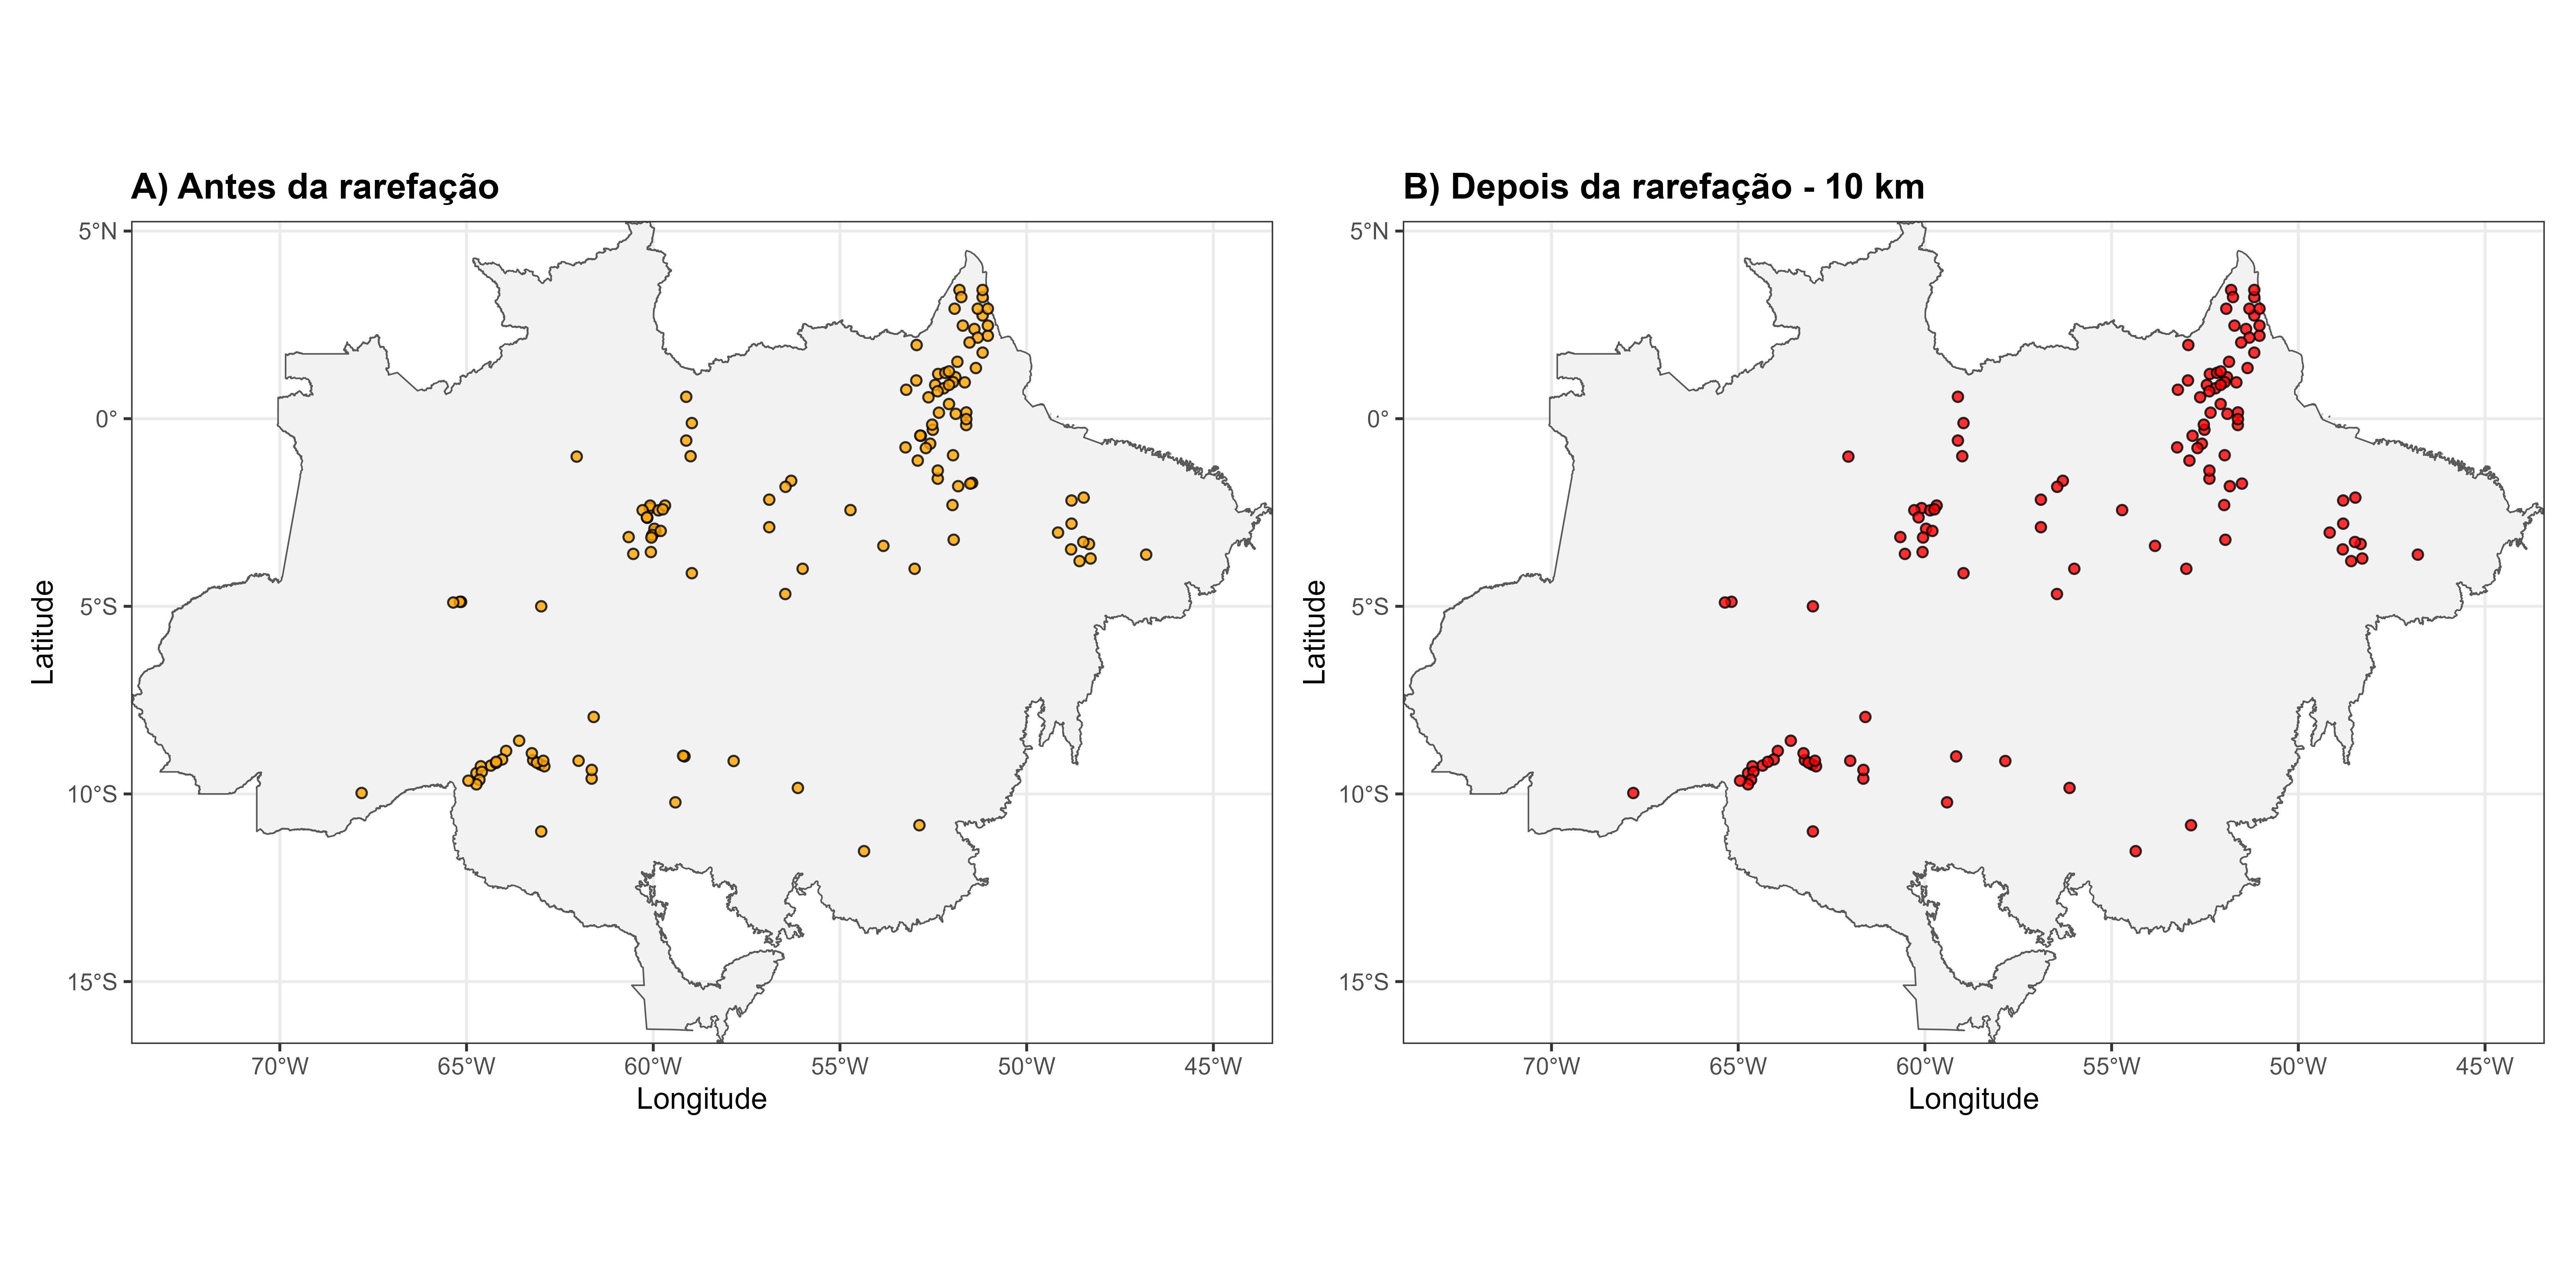
\includegraphics[width=0.92\textwidth]{figuras/unidade02/unidade02_rarefacao_dinizia.png}
	\caption{Efeito da rarefação espacial nos registros de \textit{Dinizia excelsa}. Os pontos originais apresentam concentração em determinadas regiões da Amazônia, refletindo padrões de esforço amostral. Após a aplicação do \textit{thinning}, registros espacialmente redundantes são removidos, resultando em uma distribuição mais equilibrada e adequada para modelagem.}
	\label{fig:unidade02_rarefacao_dinizia}
\end{figure}

\begin{aplicacao}[title={\faLeaf\quad Aplicação em SDM}]
	A rarefação espacial é particularmente importante em estudos que utilizam registros provenientes de herbários, plataformas globais de biodiversidade e ciência cidadã. Nessas situações, a distribuição dos dados frequentemente reflete a acessibilidade das áreas e o histórico de coleta, e não necessariamente a distribuição ecológica da espécie. A remoção de registros espacialmente redundantes contribui para reduzir esse viés e aumentar a robustez dos modelos.
\end{aplicacao}

\section{Estudo de caso: preparação dos registros de \textit{Dinizia excelsa}}

Após compreender os principais conceitos relacionados à qualidade dos dados de ocorrência, podemos agora acompanhar sua aplicação em um estudo real utilizando \textit{Dinizia excelsa} Ducke, uma das espécies arbóreas mais emblemáticas da Amazônia. Conhecida popularmente como angelim-vermelho, a espécie destaca-se por atingir grandes dimensões, elevada longevidade e ampla importância ecológica e econômica nas florestas tropicais sul-americanas.

Neste estudo de caso, os registros de ocorrência foram compilados a partir de diferentes fontes de informação, submetidos a procedimentos de controle de qualidade, filtragem espacial, rarefação e caracterização ambiental. O objetivo foi construir uma base de dados robusta e ecologicamente consistente para as etapas subsequentes de modelagem de distribuição de espécies.

\subsection{Compilação dos registros}

A primeira etapa consistiu na compilação dos registros disponíveis para \textit{Dinizia excelsa}. Os dados foram obtidos a partir de repositórios de biodiversidade e bases de dados científicas contendo registros georreferenciados da espécie em diferentes regiões da Amazônia.

A Figura \ref{fig:unidade02_mapa_ocorrencias} apresenta a distribuição inicial dos registros compilados. Observa-se uma ampla distribuição geográfica na porção norte da América do Sul, abrangendo principalmente a Amazônia brasileira e regiões adjacentes do Escudo das Guianas.

\begin{figure}[H]
	\centering
	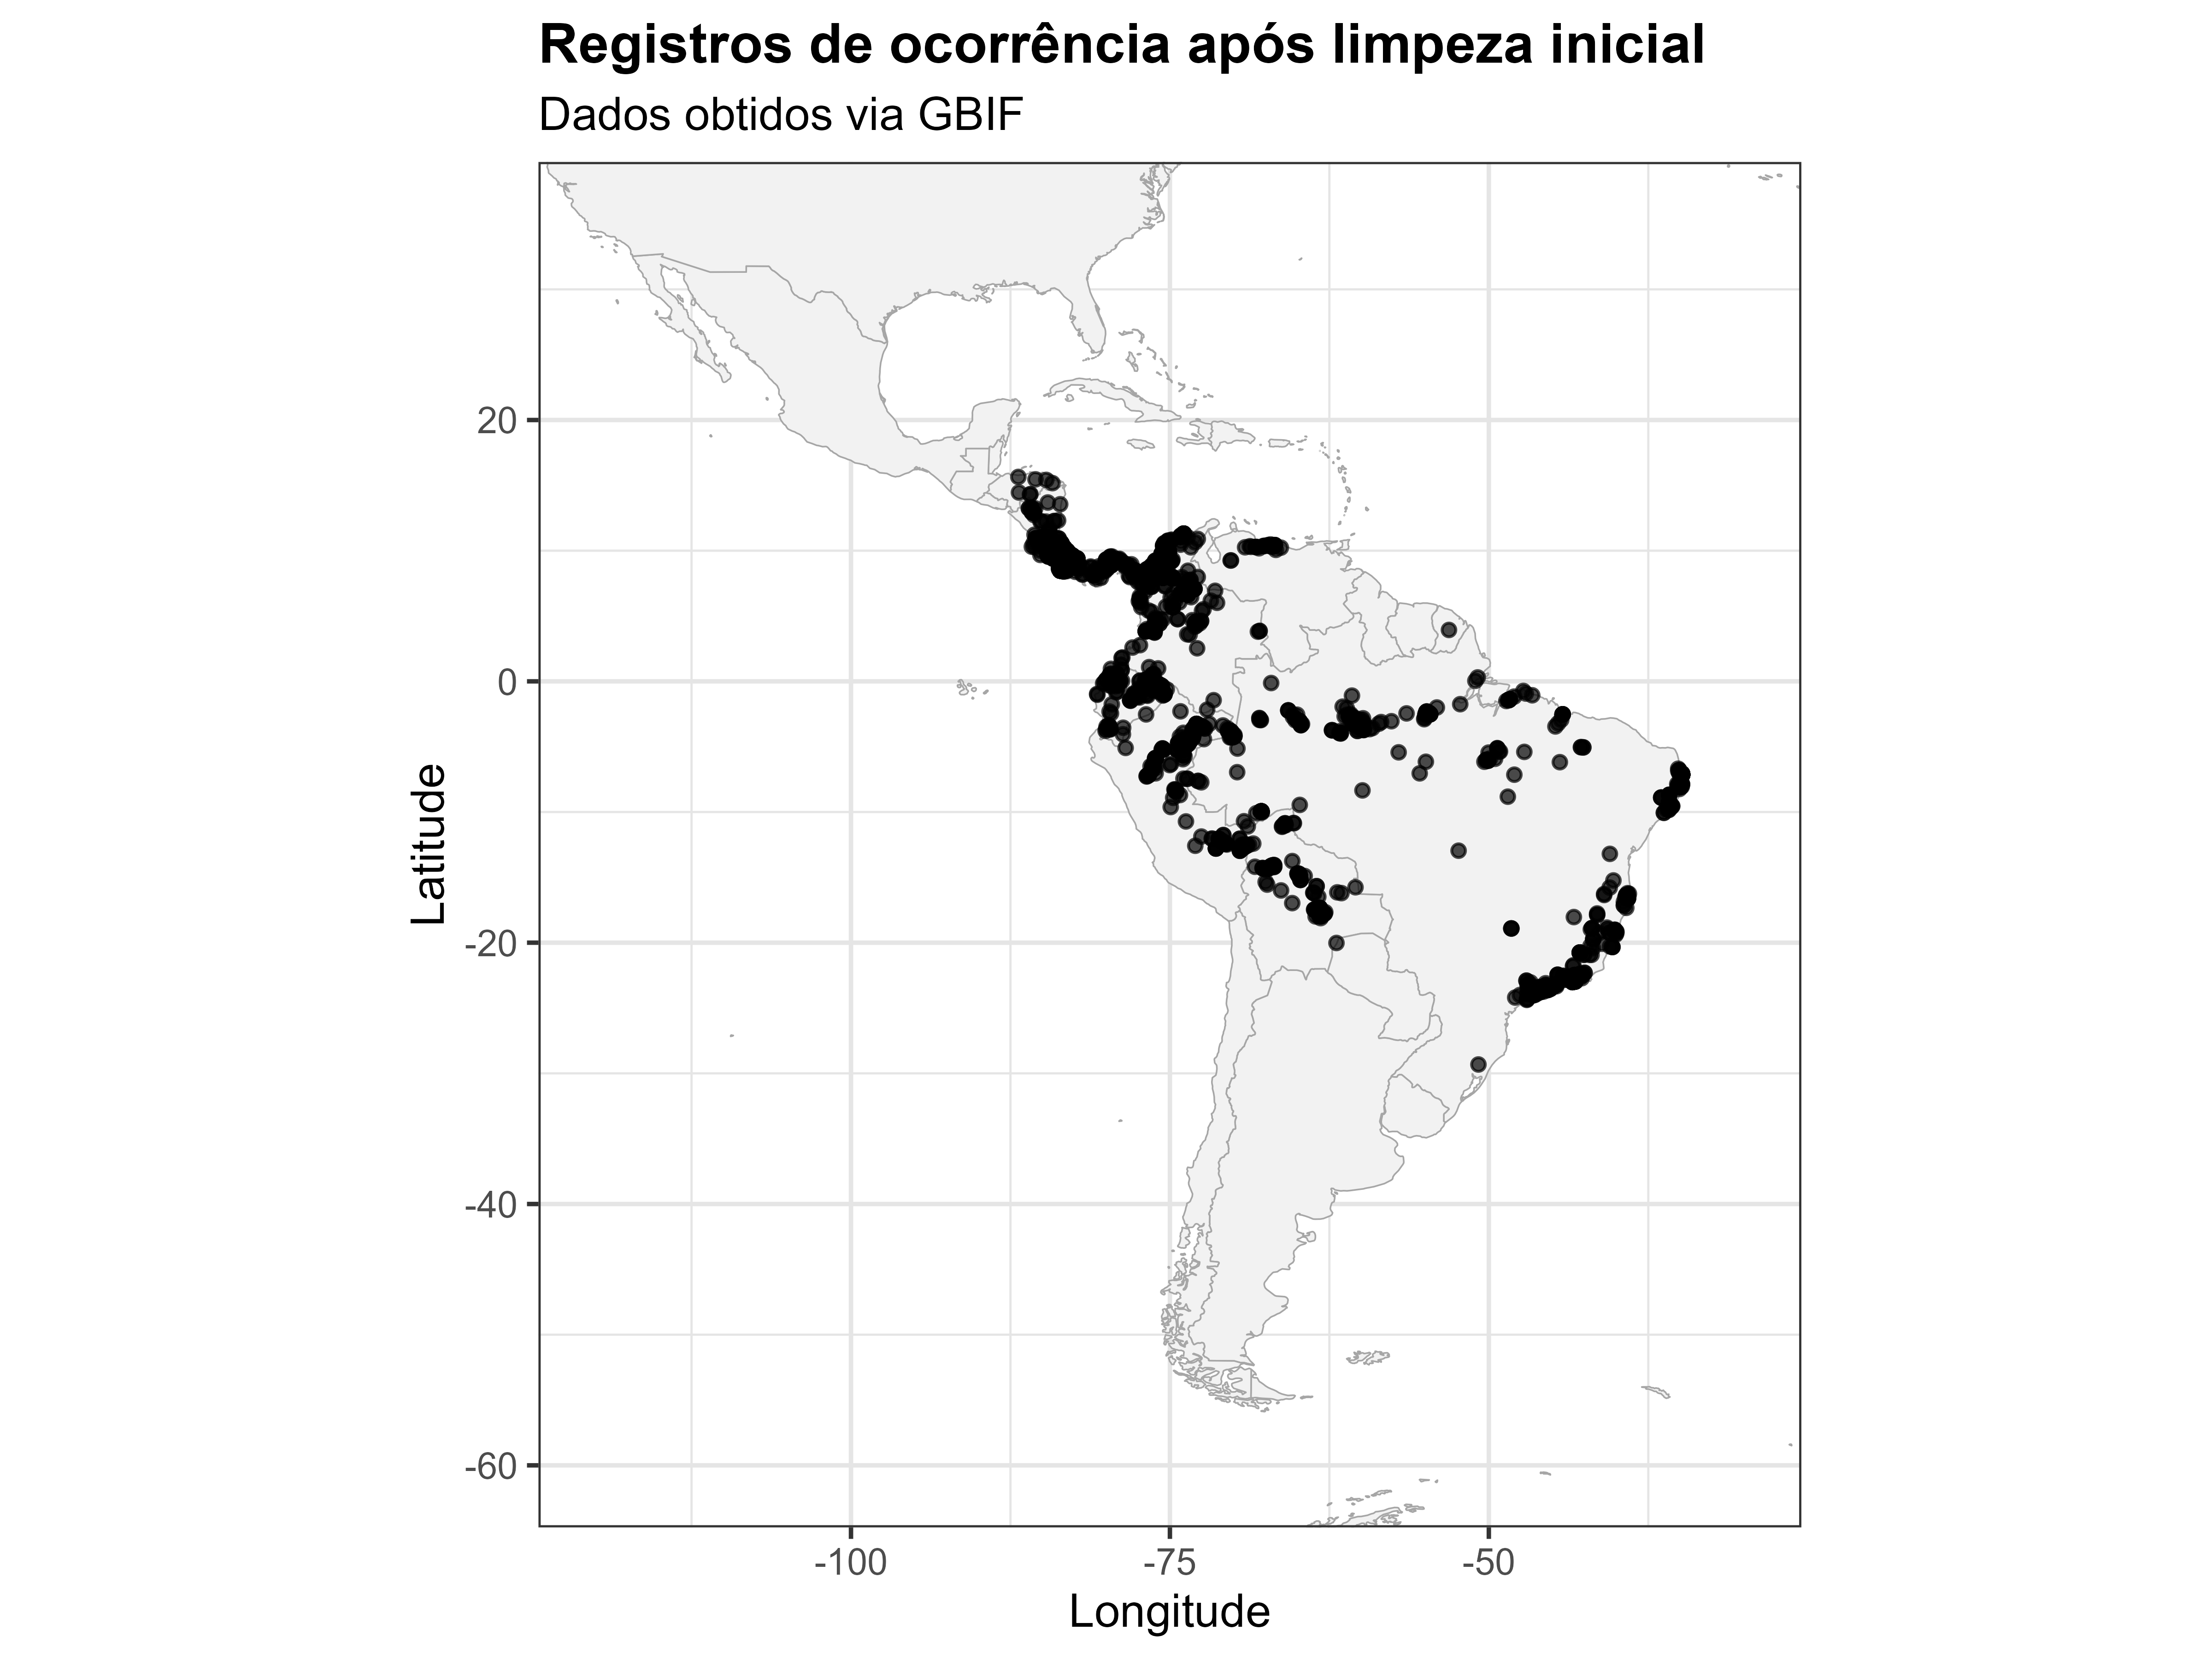
\includegraphics[width=0.92\textwidth]{figuras/unidade02/unidade02_mapa_ocorrencias.png}
	\caption{Registros de ocorrência compilados para \textit{Dinizia excelsa} utilizados neste estudo.}
	\label{fig:unidade02_mapa_ocorrencias}
\end{figure}

Embora essa distribuição forneça uma primeira aproximação da ocorrência da espécie, os registros ainda podem conter inconsistências taxonômicas, erros geográficos e redundâncias espaciais. Por essa razão, torna-se necessária uma etapa posterior de validação e limpeza dos dados.

\subsection{Limpeza e validação espacial}

Após a compilação dos registros, realizou-se um conjunto de procedimentos destinados à remoção de ocorrências problemáticas. Foram avaliadas coordenadas inválidas, registros fora da área de estudo, duplicatas geográficas e pontos potencialmente associados a erros de georreferenciamento.

A Figura \ref{fig:unidade02_bruto_limpo_dinizia} compara a distribuição dos registros antes e depois da aplicação dos filtros espaciais. Observa-se que parte das ocorrências originalmente disponíveis foi removida, resultando em uma base de dados mais coerente com a distribuição conhecida da espécie.

\begin{figure}[H]
	\centering
	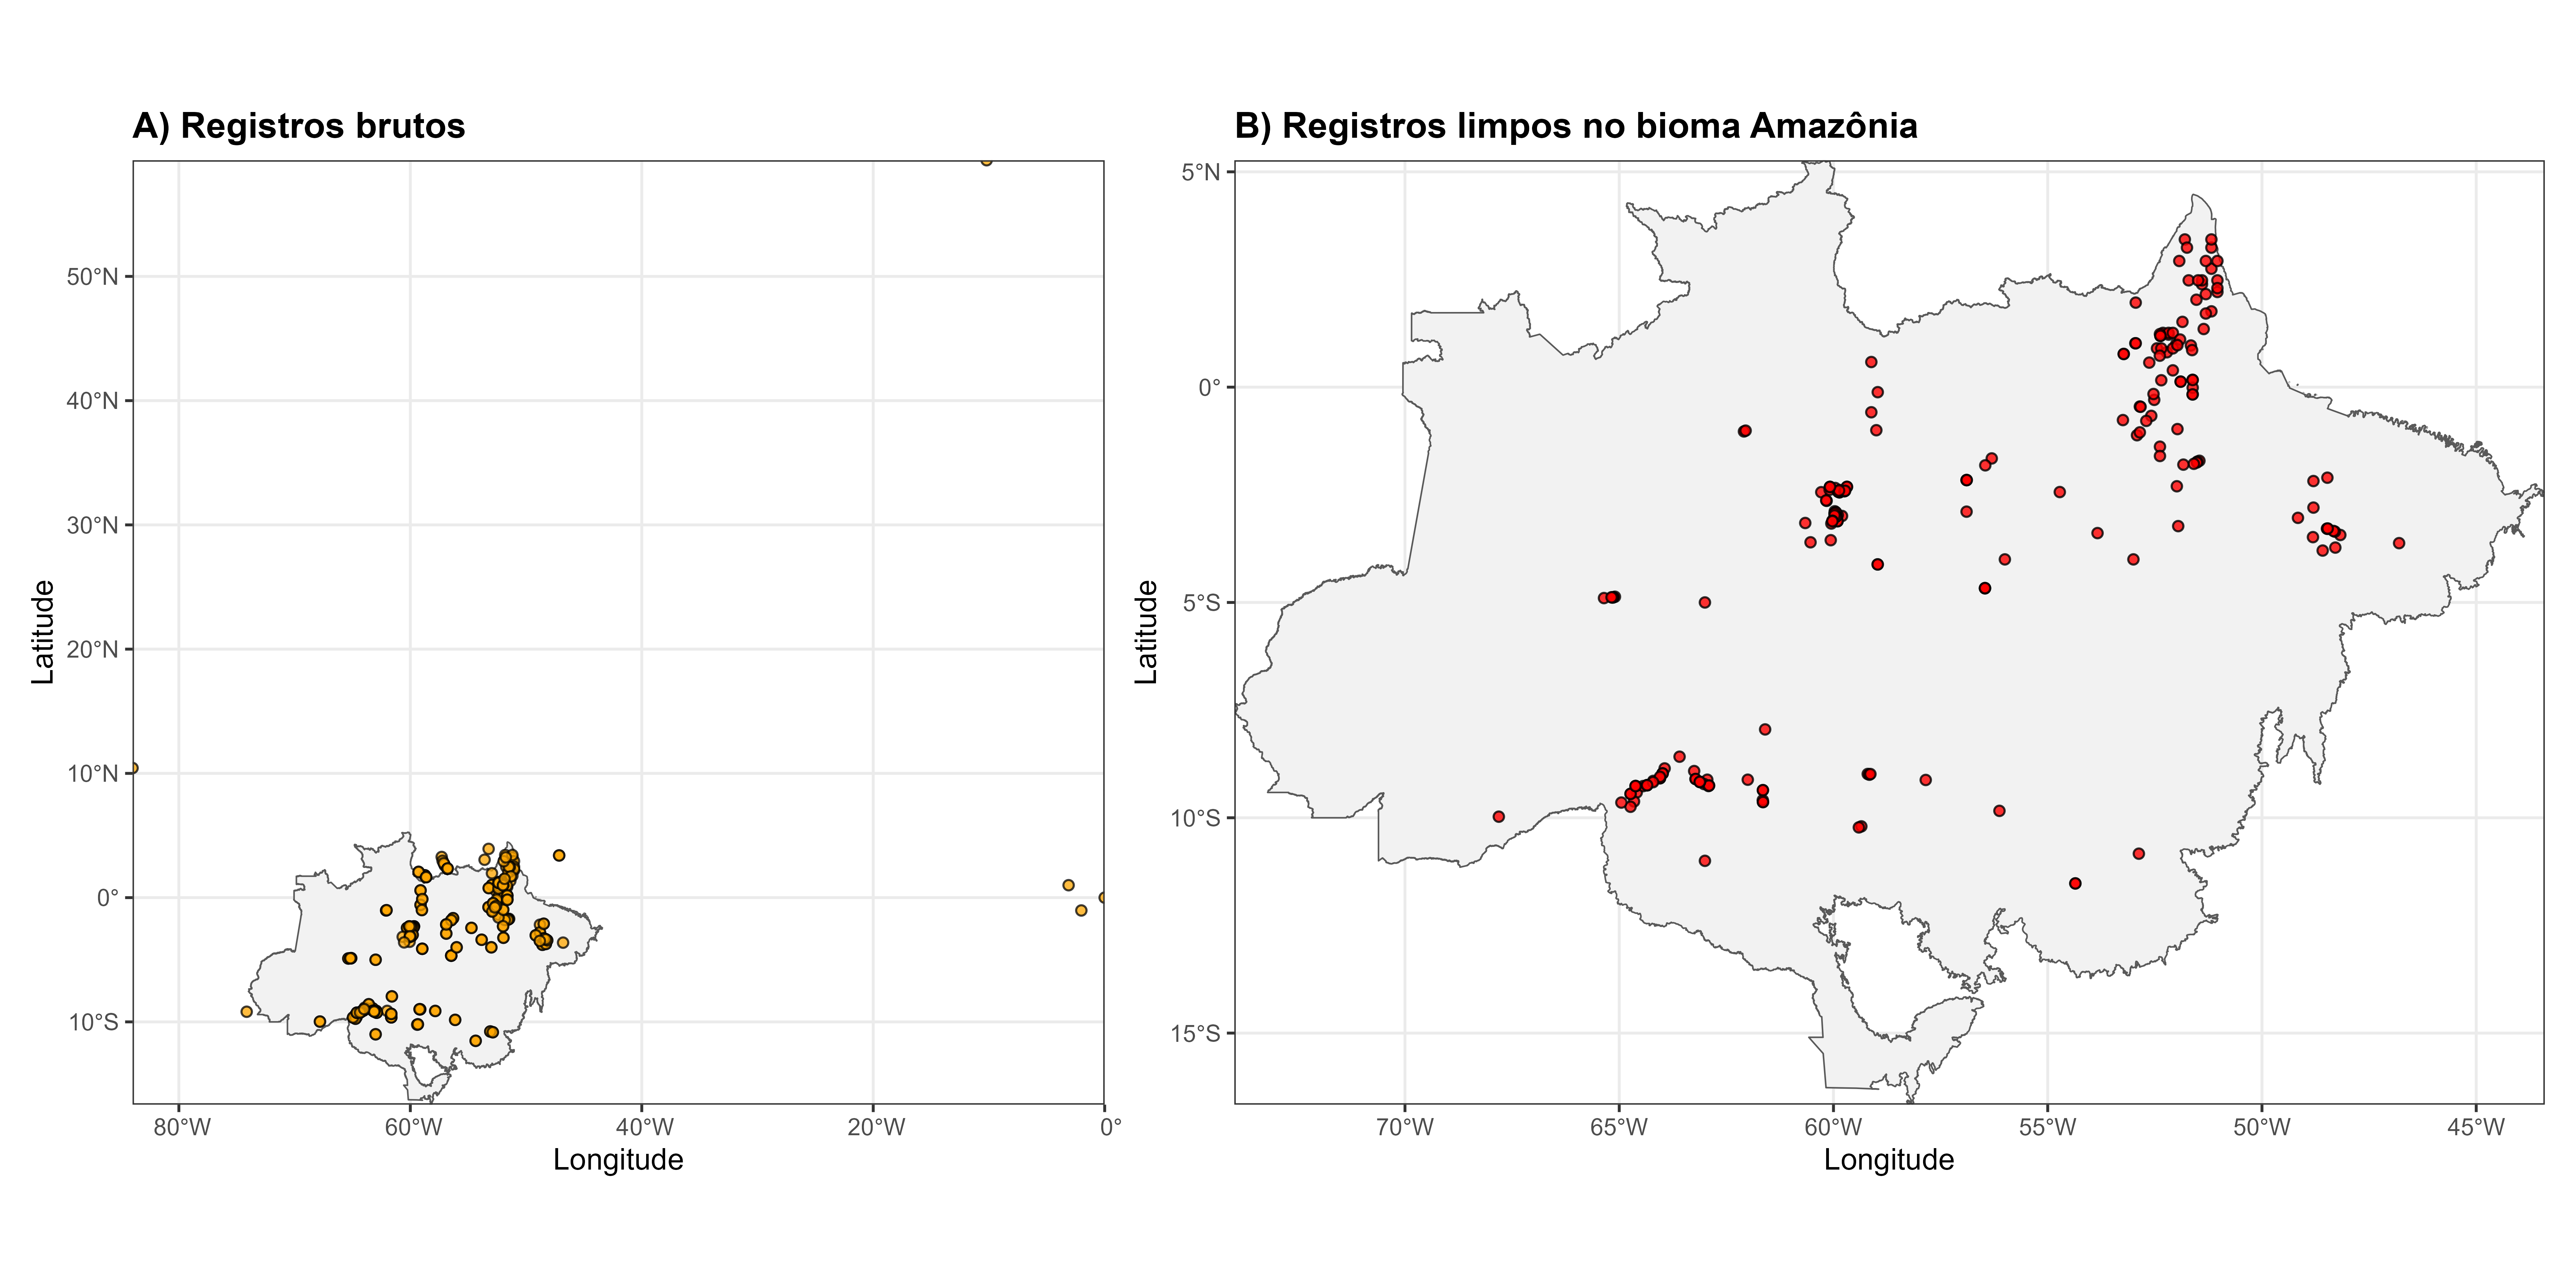
\includegraphics[width=0.92\textwidth]{figuras/unidade02/unidade02_mapa_bruto_limpo_dinizia.png}
	\caption{Comparação entre registros brutos e registros validados de \textit{Dinizia excelsa} após os procedimentos de limpeza espacial.}
	\label{fig:unidade02_bruto_limpo_dinizia}
\end{figure}

Essa etapa ilustra um princípio fundamental da SDM: a qualidade dos registros é mais importante do que sua quantidade. Um conjunto menor de ocorrências confiáveis frequentemente produz modelos mais robustos do que uma base extensa contendo erros e inconsistências.

\subsection{Rarefação espacial}

Mesmo após a limpeza geográfica, os registros ainda apresentavam concentração em determinadas regiões da Amazônia, refletindo diferenças históricas no esforço de amostragem. Para reduzir esse viés espacial, aplicou-se um procedimento de rarefação (\textit{spatial thinning}), removendo registros excessivamente próximos entre si.

A Figura \ref{fig:unidade02_rarefacao_dinizia} mostra o efeito desse procedimento sobre a distribuição espacial das ocorrências.

\begin{figure}[H]
	\centering
	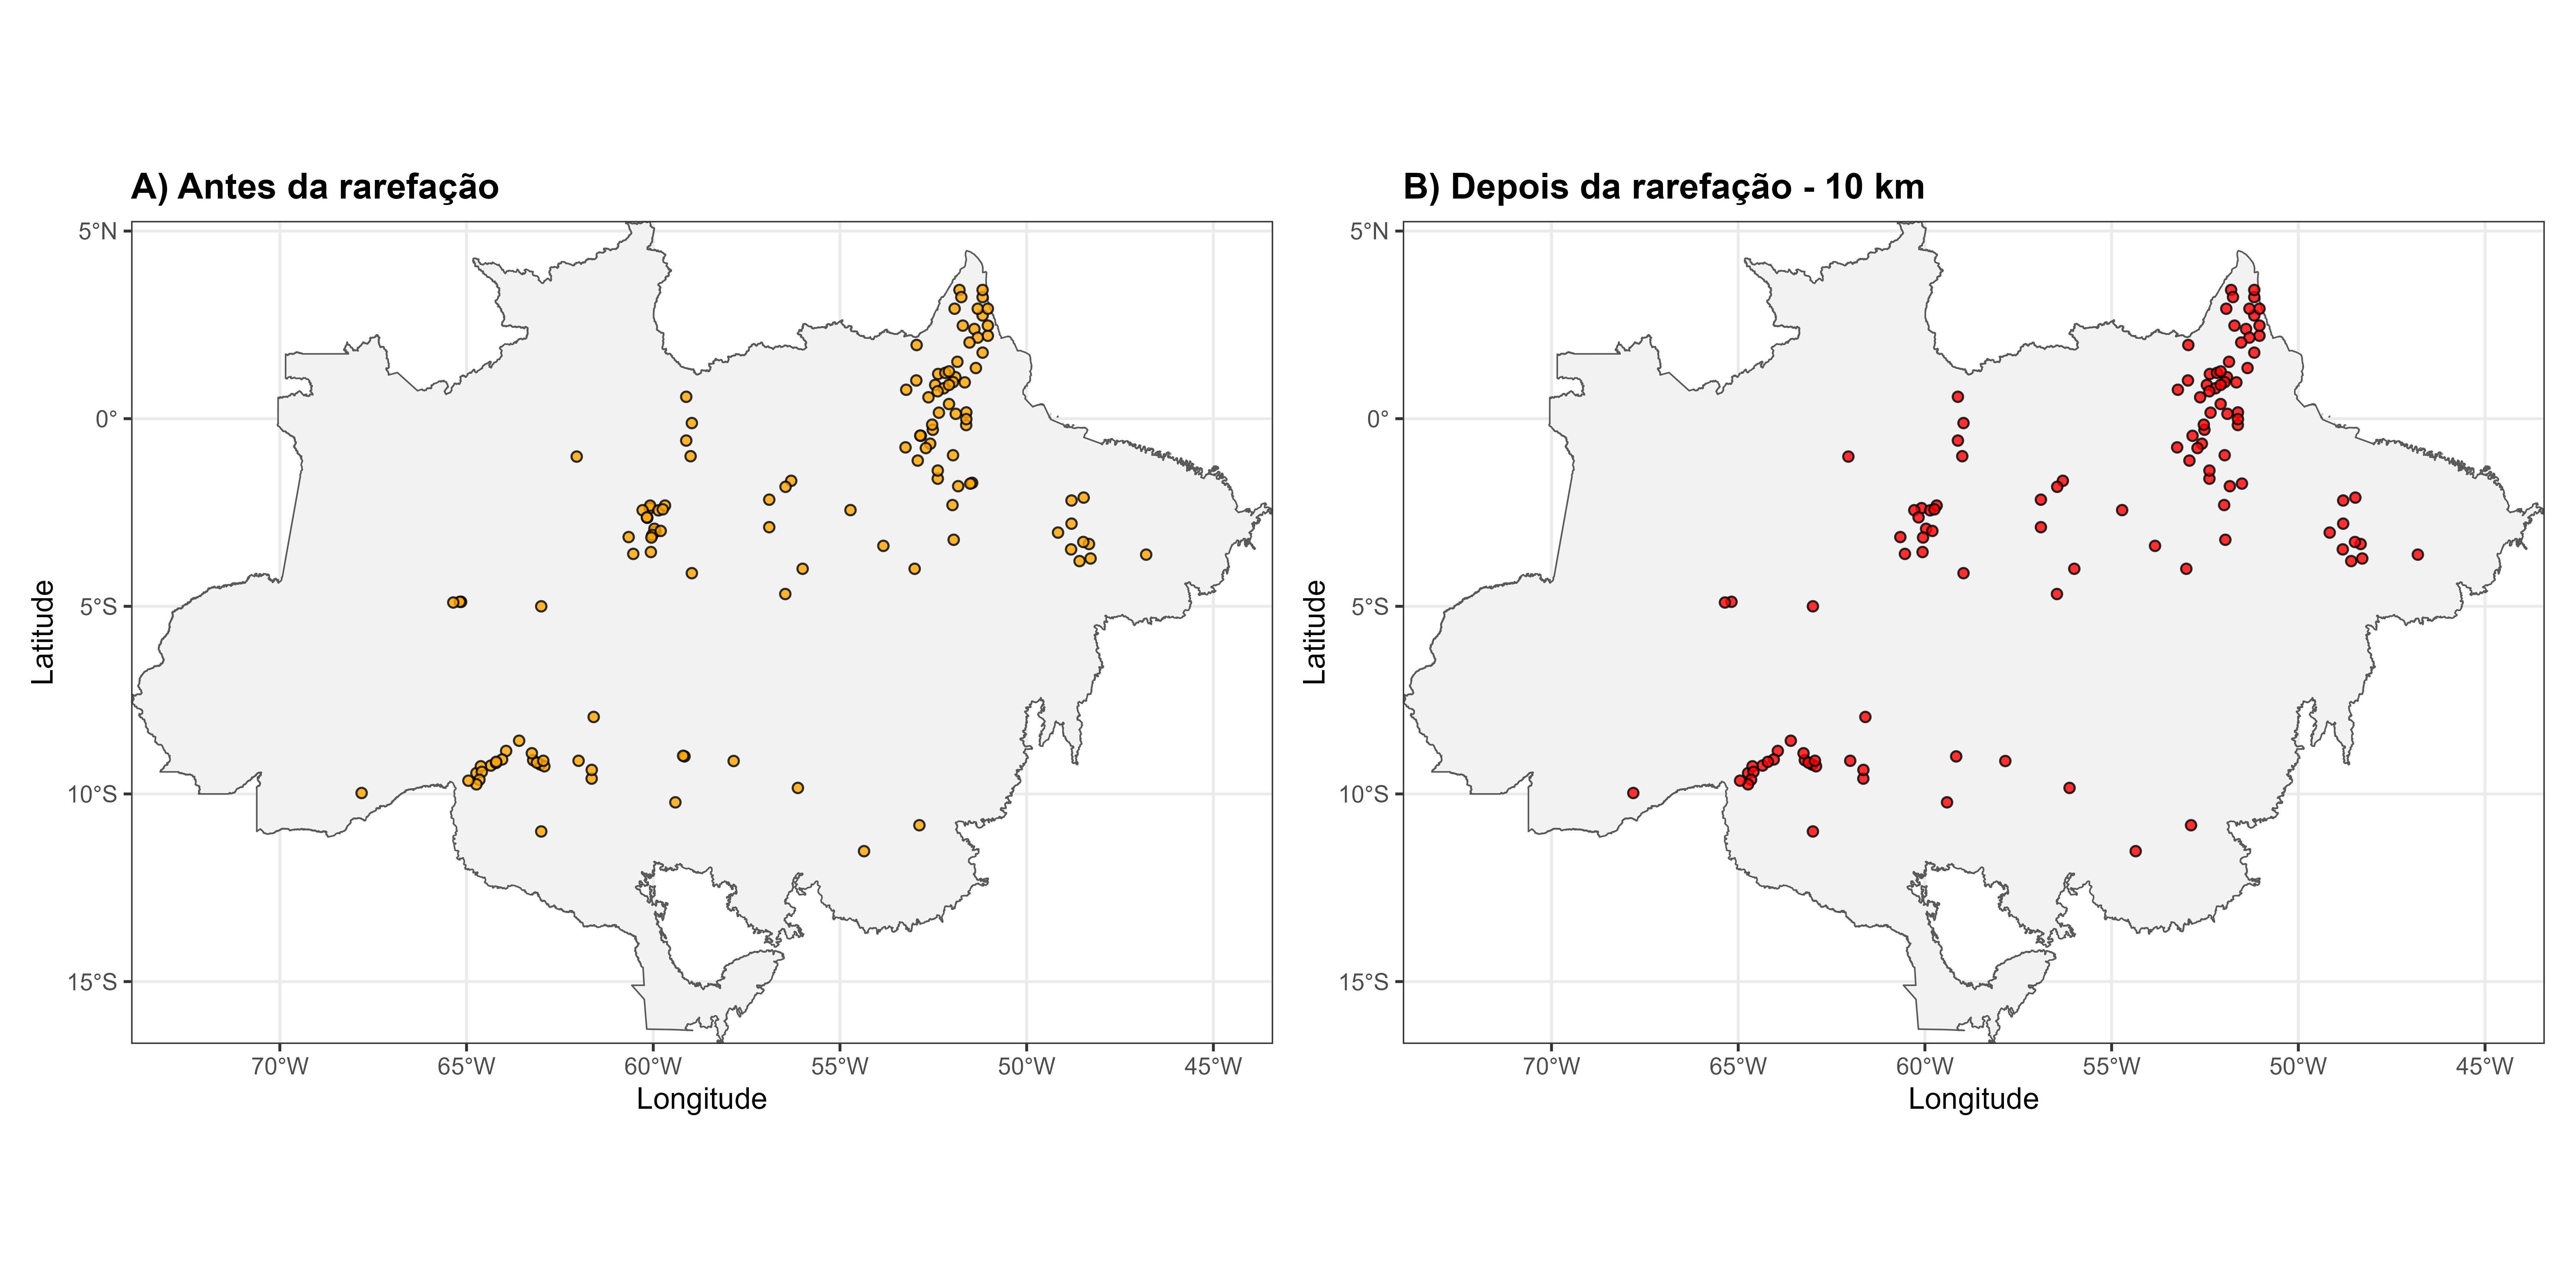
\includegraphics[width=0.92\textwidth]{figuras/unidade02/unidade02_rarefacao_dinizia.png}
	\caption{Efeito da rarefação espacial sobre os registros de \textit{Dinizia excelsa}. O procedimento reduz a redundância espacial e minimiza a influência do esforço amostral sobre a modelagem.}
	\label{fig:unidade02_rarefacao_dinizia}
\end{figure}

A rarefação não altera a distribuição geral da espécie, mas reduz a influência de áreas excessivamente amostradas, contribuindo para uma representação mais equilibrada do nicho ecológico ocupado pela espécie.

\subsection{Extração das variáveis ambientais}

Uma vez obtida a base final de ocorrências, cada registro foi associado às condições ambientais presentes no local de ocorrência. Para isso, foram extraídas variáveis bioclimáticas derivadas de camadas ambientais em resolução compatível com a escala do estudo.

A Figura \ref{fig:unidade02_hist_variaveis_dinizia} apresenta a distribuição dos valores observados para algumas das variáveis utilizadas na modelagem.

\begin{figure}[H]
	\centering
	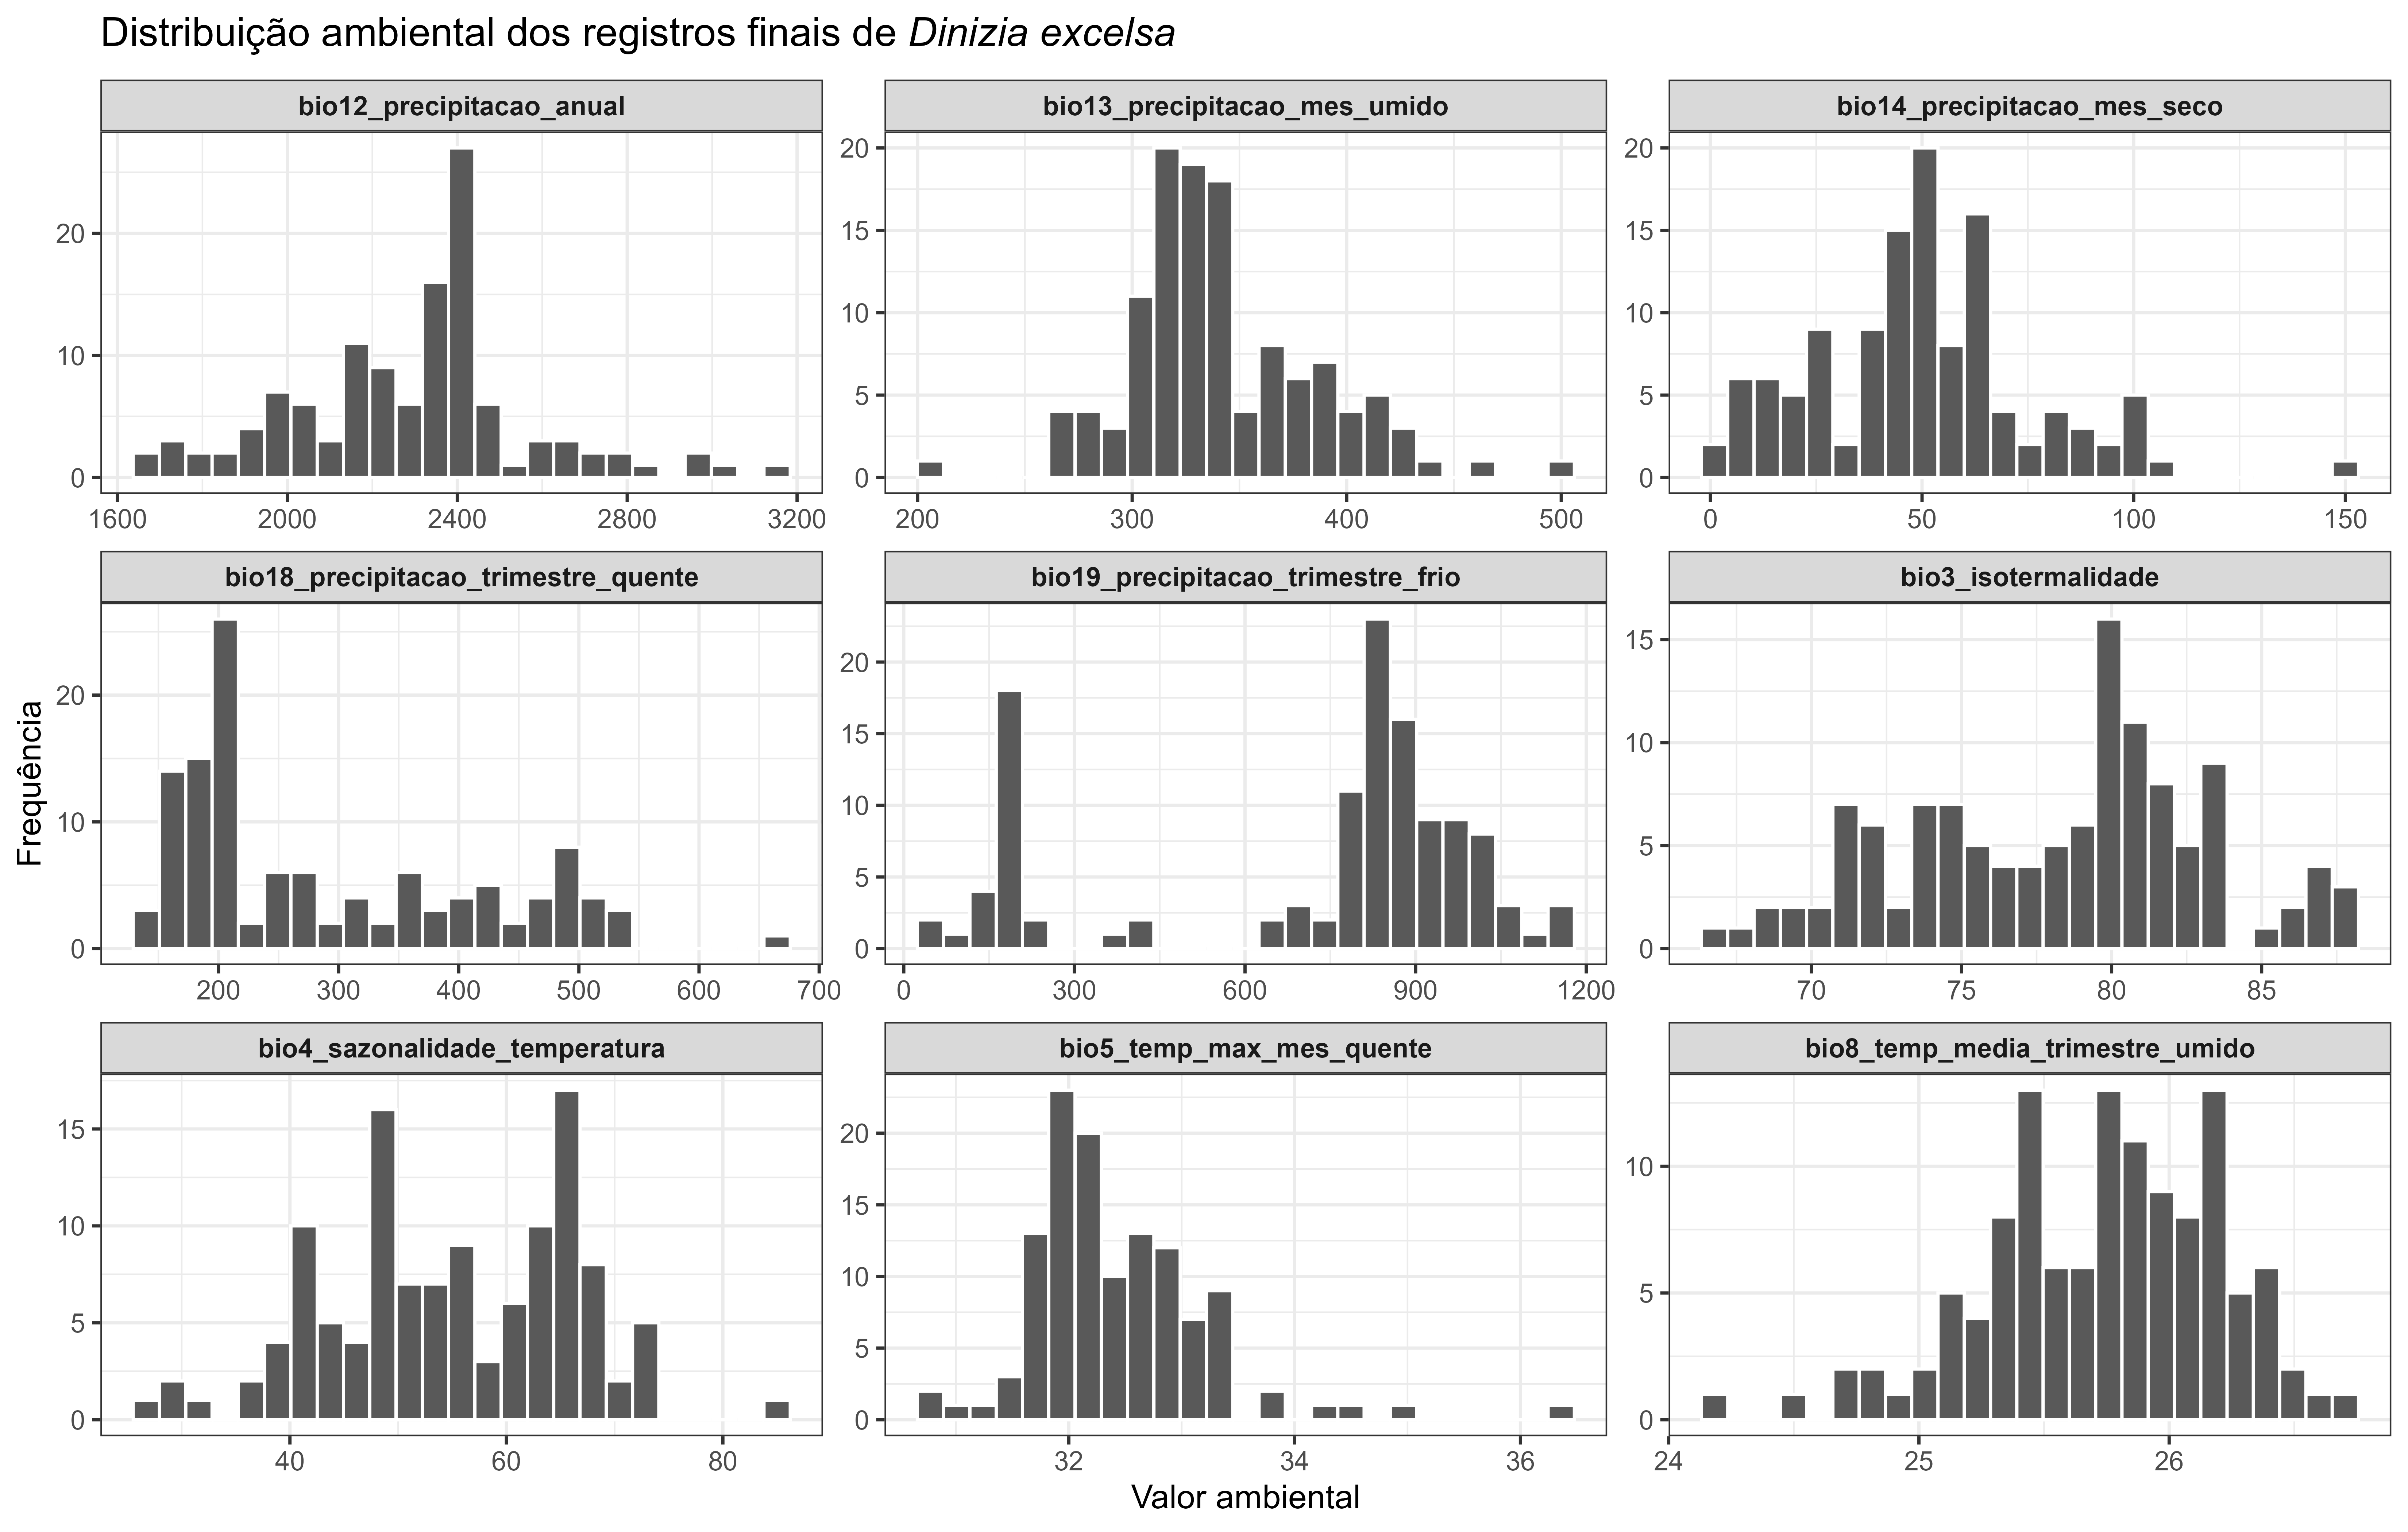
\includegraphics[width=0.92\textwidth]{figuras/unidade02/unidade02_histogramas_variaveis_dinizia.png}
	\caption{Distribuição das variáveis ambientais associadas aos registros de \textit{Dinizia excelsa}.}
	\label{fig:unidade02_hist_variaveis_dinizia}
\end{figure}

A análise dessas distribuições fornece uma primeira visão da amplitude ambiental ocupada pela espécie e permite identificar possíveis valores extremos, lacunas amostrais ou padrões ecológicos relevantes para a modelagem.

\subsection{Caracterização do nicho climático ocupado}

Além de analisar cada variável isoladamente, é possível investigar simultaneamente as condições ambientais ocupadas pela espécie em relação ao conjunto de ambientes disponíveis na Amazônia.

A Figura \ref{fig:unidade02_espaco_climatico_dinizia} apresenta uma representação do espaço climático ocupado por \textit{Dinizia excelsa} em comparação com o background ambiental do bioma Amazônia.

\begin{figure}[H]
	\centering
	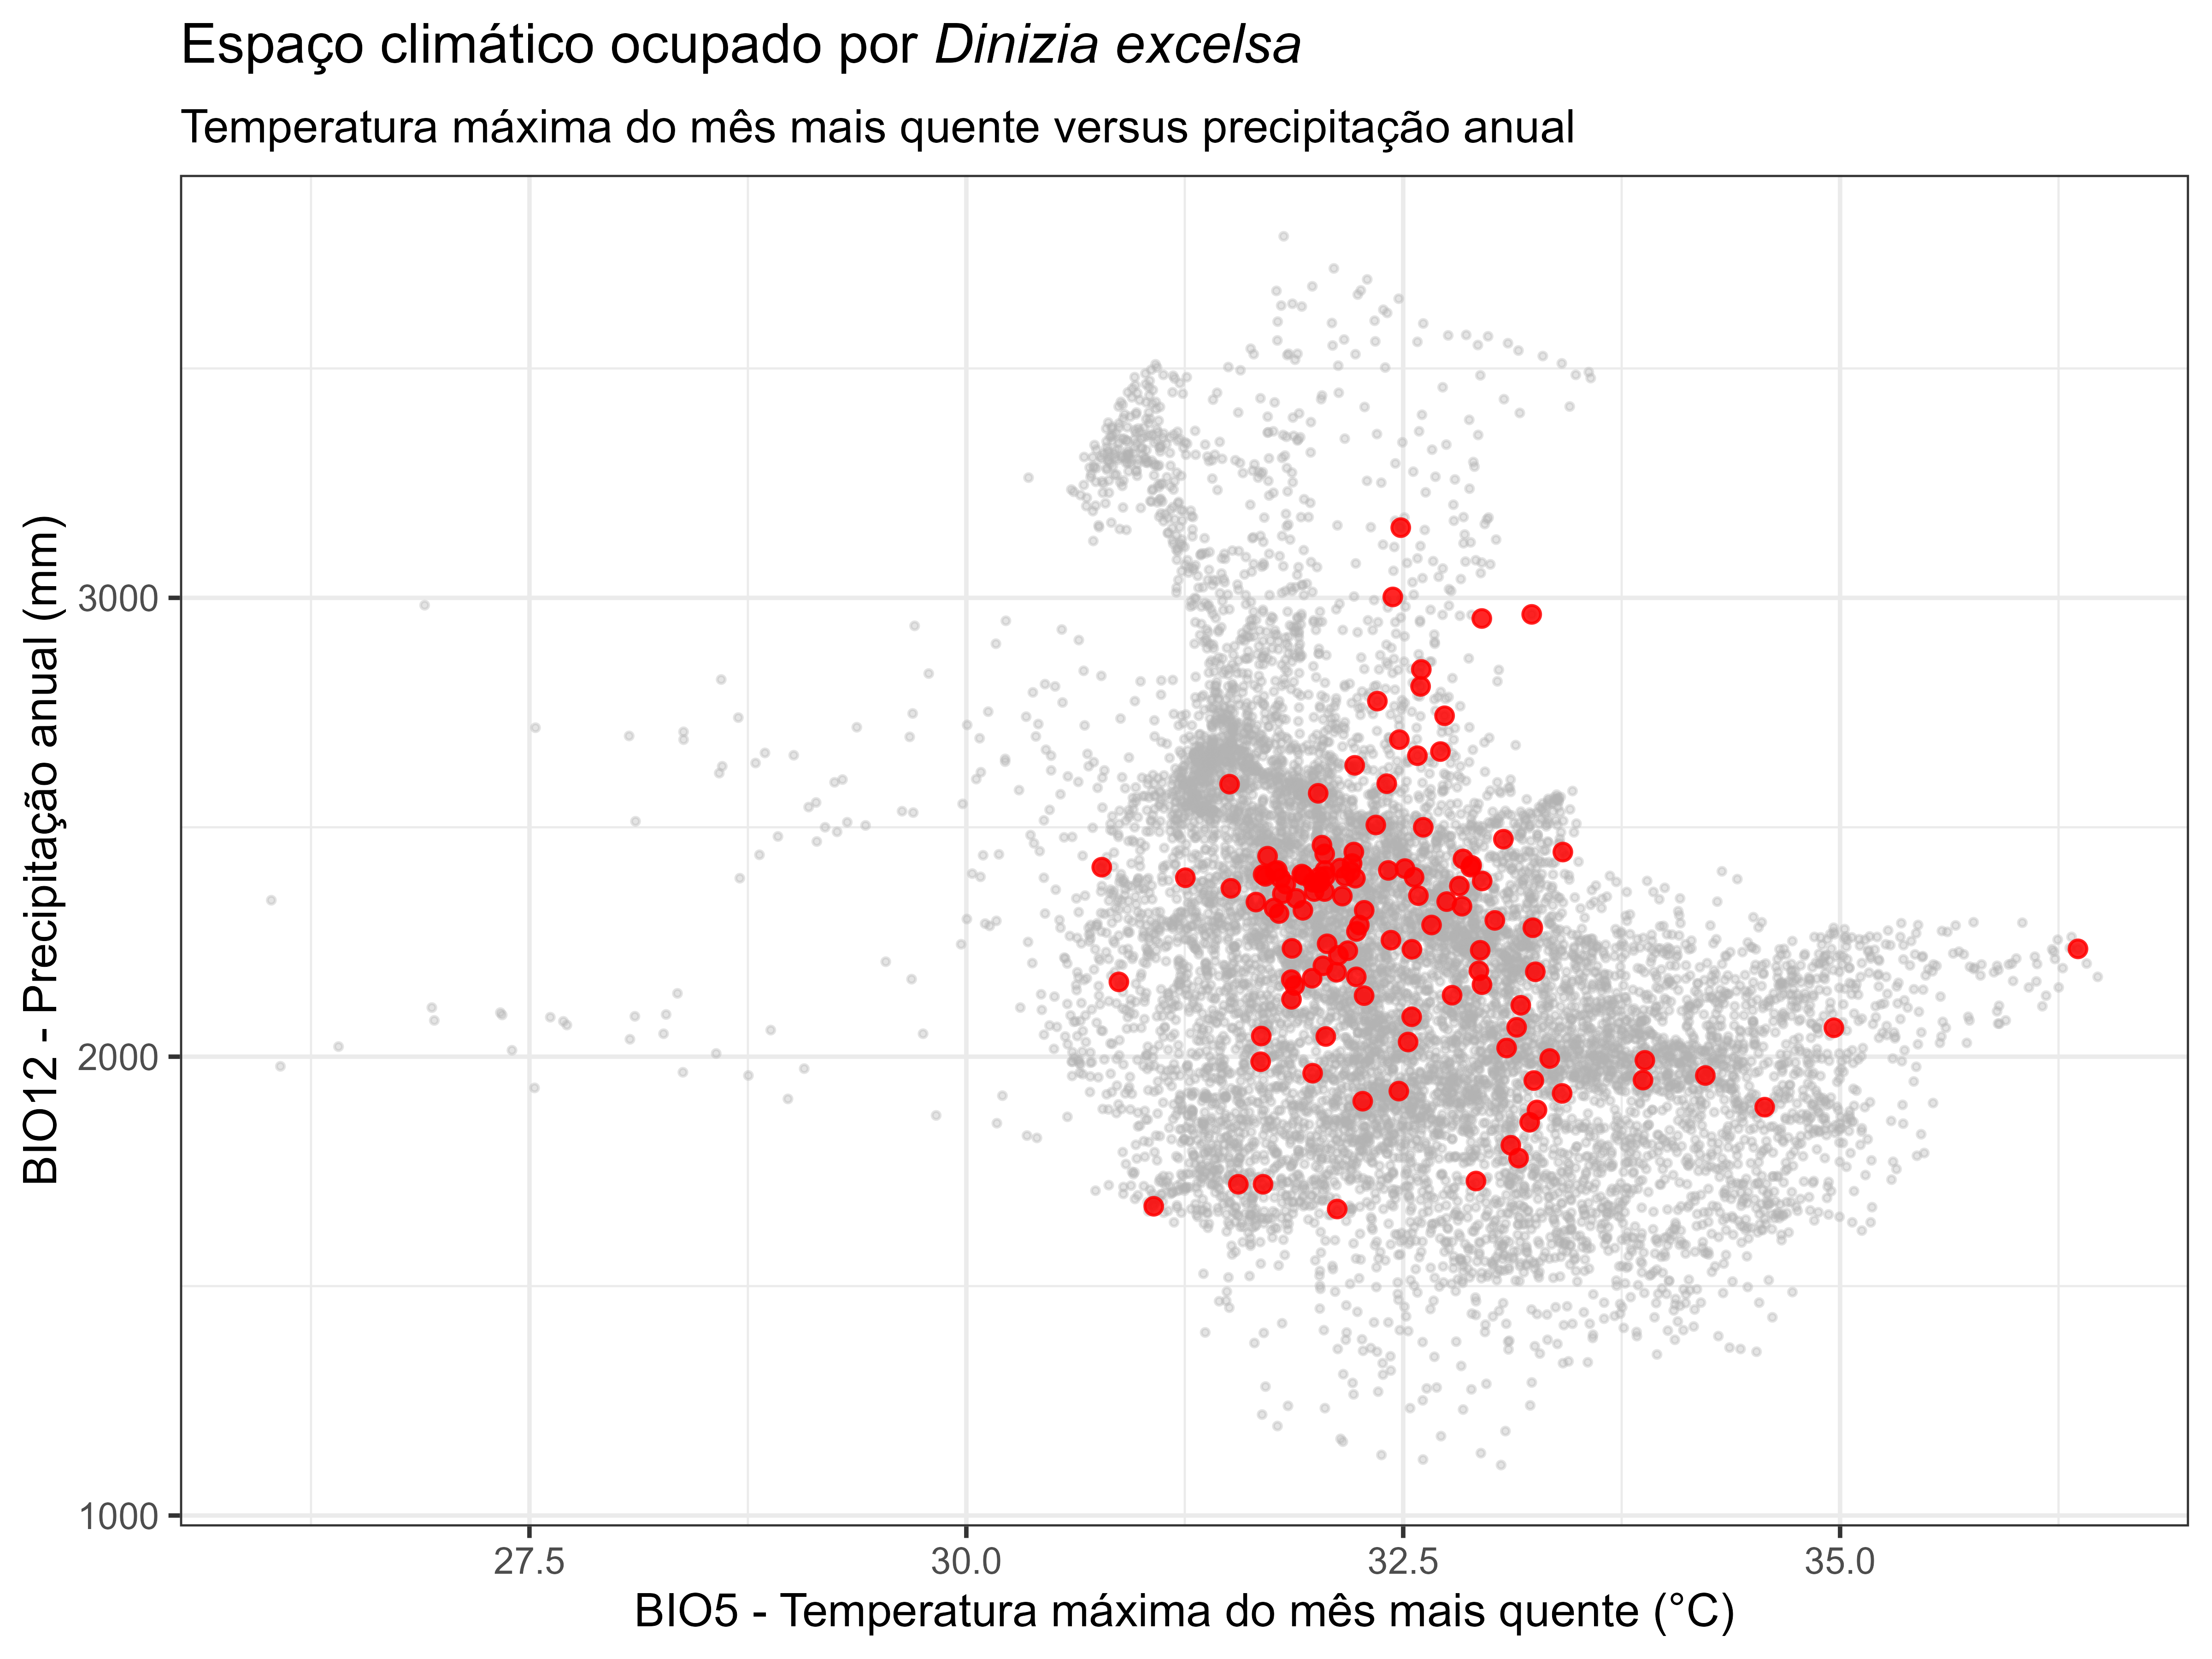
\includegraphics[width=0.86\textwidth]{figuras/unidade02/unidade02_espaco_climatico_dinizia.png}
	\caption{Espaço climático ocupado por \textit{Dinizia excelsa} em relação ao conjunto de condições ambientais disponíveis no bioma Amazônia.}
	\label{fig:unidade02_espaco_climatico_dinizia}
\end{figure}

Essa figura possui importância central para a compreensão dos fundamentos ecológicos da Modelagem de Distribuição de Espécies. Observa-se que os registros de \textit{Dinizia excelsa} ocupam apenas uma fração do espaço climático disponível na Amazônia. Embora o bioma apresente ampla heterogeneidade ambiental, a espécie encontra-se associada a um subconjunto relativamente específico de condições climáticas.

De maneira geral, os registros concentram-se em regiões caracterizadas por precipitações anuais elevadas, geralmente entre aproximadamente 1.800 e 3.000 mm por ano, e temperaturas máximas do mês mais quente próximas de 31,5 a 33,5,°C. Esses padrões sugerem que a espécie não utiliza todo o espectro climático disponível no bioma, mas ocupa um conjunto mais restrito de condições ambientais compatíveis com suas exigências ecológicas.

Esse resultado ilustra de forma prática a distinção entre espaço geográfico e espaço ambiental discutida na Unidade 01. Enquanto a Amazônia ocupa uma extensa região geográfica contendo grande diversidade de condições climáticas, \textit{Dinizia excelsa} utiliza apenas parte desse espaço ambiental. Em outras palavras, sua distribuição observada representa uma amostra do nicho realizado da espécie.

Além disso, essa análise antecipa conceitos que serão aprofundados nas próximas unidades. Na Unidade 03 discutiremos como delimitar a área acessível (M), distinguindo ambientes disponíveis daqueles efetivamente acessíveis à espécie. Na Unidade 04 abordaremos a estrutura de correlação entre as variáveis ambientais que definem esse espaço climático. Assim, o conjunto de registros preparado nesta unidade constitui a base empírica sobre a qual todas as etapas posteriores de modelagem serão construídas.

\begin{conceito}[title={\faBook\quad Integração conceitual}]
	Os registros de ocorrência representam observações do nicho realizado da espécie. Após os procedimentos de limpeza, rarefação e caracterização ambiental, esses registros tornam-se a principal fonte de informação utilizada para inferir as relações entre a espécie e o ambiente em modelos de distribuição.
\end{conceito}


\begin{table}[H]
	\centering
	\caption{Resumo das etapas de preparação dos registros de \textit{Dinizia excelsa} para Modelagem de Distribuição de Espécies.}
	\label{tab:fluxo_preparacao_dinizia}
	\begin{tabular}{p{3.2cm}p{5.2cm}p{5.2cm}}
		\toprule
		\textbf{Etapa} &
		\textbf{Objetivo} &
		\textbf{Produto gerado} \\
		\midrule
		
		Compilação dos registros
		&
		Reunir ocorrências provenientes de diferentes fontes de dados biológicos.
		&
		Base inicial de registros georreferenciados da espécie.
		
		\\
		
		Limpeza e validação espacial
		&
		Remover coordenadas inválidas, registros inconsistentes e ocorrências fora da área de estudo.
		&
		Base validada e espacialmente coerente.
		
		\\
		
		Rarefação espacial
		&
		Reduzir redundâncias espaciais e minimizar efeitos do viés amostral.
		&
		Conjunto de ocorrências espacialmente mais independente.
		
		\\
		
		Extração ambiental
		&
		Associar cada ocorrência às condições ambientais presentes no local de registro.
		&
		Matriz espécie--ambiente para análises ecológicas.
		
		\\
		
		Caracterização do nicho climático
		&
		Identificar as condições ambientais efetivamente ocupadas pela espécie.
		&
		Representação do espaço climático ocupado por \textit{Dinizia excelsa}.
		
		\\
		
		Preparação para SDM
		&
		Construir uma base de dados adequada para as etapas de modelagem.
		&
		Conjunto final de ocorrências utilizado nas unidades seguintes.
		
		\\
		
		\bottomrule
	\end{tabular}
\end{table}

\section{Fluxograma completo de preparação dos dados}

As etapas apresentadas ao longo desta unidade podem ser organizadas em um fluxo lógico de trabalho que transforma registros brutos de ocorrência em uma base de dados adequada para Modelagem de Distribuição de Espécies. Embora diferentes estudos possam adotar procedimentos específicos de acordo com seus objetivos, a sequência geral de compilação, validação, filtragem, rarefação e caracterização ambiental representa atualmente uma das abordagens mais utilizadas em pesquisas de SDM \parencite{guisan2017habitat,peterson2011ecological}.

O fluxograma apresentado na Figura \ref{fig:unidade02_fluxograma_dinizia} sintetiza o pipeline aplicado aos registros de \textit{Dinizia excelsa} ao longo desta unidade. O processo inicia com a compilação dos dados provenientes de diferentes fontes, seguida pela padronização taxonômica e geográfica dos registros. Em seguida, são realizados procedimentos de controle de qualidade destinados à remoção de coordenadas problemáticas, registros duplicados e ocorrências inconsistentes. Após a rarefação espacial, os registros remanescentes são associados às variáveis ambientais, resultando em uma base final pronta para as etapas subsequentes de modelagem.

\begin{figure}[H]
	\centering
	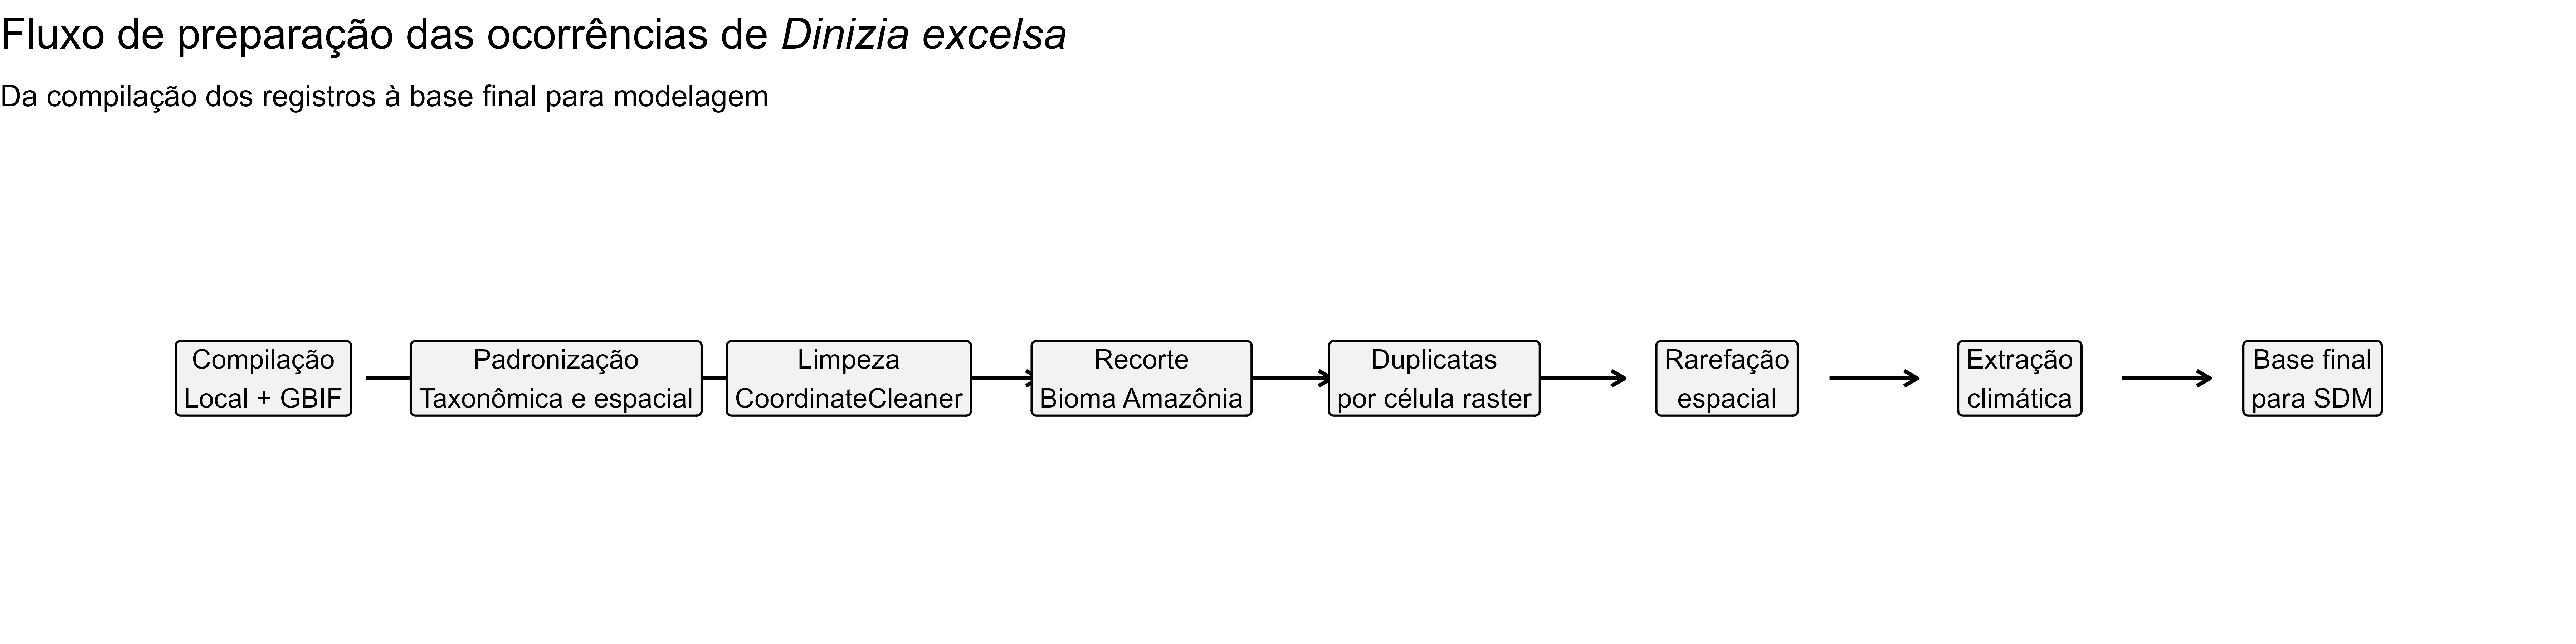
\includegraphics[width=0.92\textwidth]{figuras/unidade02/unidade02_fluxograma_preparacao_dinizia.png}
	\caption{Fluxograma geral de preparação dos registros de ocorrência de \textit{Dinizia excelsa} para Modelagem de Distribuição de Espécies.}
	\label{fig:unidade02_fluxograma_dinizia}
\end{figure}

É importante observar que a preparação dos dados não deve ser encarada como uma etapa meramente técnica. Cada decisão tomada durante esse processo influencia diretamente a representação do nicho ecológico da espécie e, consequentemente, os resultados obtidos pelos modelos. Assim, a construção de uma base de dados confiável constitui um componente fundamental da inferência ecológica em SDM.

\section{Boas práticas em dados de ocorrência para SDM}

A crescente disponibilidade de registros biológicos ampliou significativamente as possibilidades de aplicação da Modelagem de Distribuição de Espécies. Entretanto, o uso adequado desses dados exige uma postura crítica em relação à sua qualidade e representatividade. A simples obtenção de grandes quantidades de registros não garante a construção de modelos robustos ou ecologicamente coerentes.

Em estudos de SDM, a qualidade dos registros deve sempre prevalecer sobre a quantidade de ocorrências disponíveis. Procedimentos de validação taxonômica, verificação geográfica, remoção de duplicatas e avaliação de vieses espaciais devem ser incorporados rotineiramente ao fluxo de trabalho. Da mesma forma, todas as etapas de processamento precisam ser documentadas de forma transparente, garantindo a reprodutibilidade das análises e permitindo futuras revisões dos resultados \parencite{zurell2020standard,guisan2017habitat}.

A Tabela \ref{tab:boas_praticas_ocorrencias} resume alguns dos problemas mais frequentes encontrados em bases de ocorrência e as estratégias normalmente utilizadas para sua correção ou mitigação.


\begin{table}[H]
	\centering
	\caption{Problemas frequentes em dados de ocorrência e estratégias recomendadas para sua correção ou mitigação.}
	\label{tab:boas_praticas_ocorrencias}
	\begin{tabular}{p{4cm}p{5cm}p{5cm}}
		\toprule
		\textbf{Problema} &
		\textbf{Consequência} &
		\textbf{Solução recomendada} \\
		\midrule
		
		Coordenadas inválidas
		&
		Extração incorreta de variáveis ambientais.
		&
		Validação geográfica e uso do \texttt{CoordinateCleaner}.
		
		\\
		
		Erros taxonômicos
		&
		Associação equivocada entre espécie e ambiente.
		&
		Padronização nomenclatural e revisão taxonômica.
		
		\\
		
		Duplicatas geográficas
		&
		Redundância de informações espaciais.
		&
		Remoção de registros repetidos.
		
		\\
		
		Duplicatas por célula raster
		&
		Pseudorreplicação ambiental.
		&
		Manter apenas um registro por pixel ambiental.
		
		\\
		
		Registros institucionais
		&
		Concentração artificial de ocorrências.
		&
		Filtragem automática e inspeção visual.
		
		\\
		
		Registros ex situ
		&
		Representação inadequada do nicho natural.
		&
		Remoção de jardins botânicos e arboretos.
		
		\\
		
		Viés espacial de amostragem
		&
		Superestimação de áreas intensamente amostradas.
		&
		Rarefação espacial (\textit{thinning}).
		
		\\
		
		Baixa precisão espacial
		&
		Incerteza na associação espécie--ambiente.
		&
		Avaliação da qualidade e exclusão de registros problemáticos.
		
		\\
		
		\bottomrule
	\end{tabular}
\end{table}

\section{Estudo integrador: construindo uma base de dados confiável para modelar a distribuição de \textit{Dinizia excelsa}}

Ao longo das Unidades 01 e 02, acompanhamos dois componentes fundamentais da Modelagem de Distribuição de Espécies. Na primeira unidade, discutimos os fundamentos ecológicos do nicho, explorando como fatores ambientais, interações bióticas e processos históricos influenciam a distribuição das espécies. Nesta unidade, voltamos nossa atenção para a principal evidência empírica utilizada para representar esses processos: os registros de ocorrência.

A preparação dos dados de \textit{Dinizia excelsa} ilustra como conceitos ecológicos e procedimentos metodológicos estão intimamente conectados. Os registros compilados a partir de herbários, coleções biológicas e bancos de dados globais representam observações do nicho realizado da espécie. Entretanto, para que essas observações possam ser utilizadas em SDM, é necessário garantir que reflitam adequadamente os ambientes efetivamente ocupados pela espécie.

A limpeza taxonômica e geográfica reduz inconsistências capazes de distorcer as relações entre ocorrência e ambiente. A rarefação espacial minimiza a influência do esforço amostral sobre a distribuição dos registros. A extração das variáveis ambientais, por sua vez, permite caracterizar o conjunto de condições climáticas associado às ocorrências observadas. Como resultado, obtém-se uma representação mais fiel do nicho ecológico ocupado por \textit{Dinizia excelsa} na Amazônia.

Entretanto, ainda existe uma questão fundamental a ser respondida: quais ambientes estavam efetivamente disponíveis para a espécie ao longo de sua história evolutiva? Nem toda região ambientalmente adequada é necessariamente acessível a uma espécie. Barreiras geográficas, limitações de dispersão e processos históricos restringem os ambientes que podem ser ocupados ao longo do tempo.

Essa questão conduz diretamente ao próximo passo do processo de modelagem. Na Unidade 03, introduziremos o conceito de área acessível (M), componente central do framework BAM e um dos elementos mais importantes para a construção de modelos ecologicamente realistas. Antes de modelar onde uma espécie pode ocorrer, é necessário compreender quais ambientes ela teve oportunidade de alcançar.

Os conceitos apresentados nesta unidade estabelecem os fundamentos necessários para a construção de bases de ocorrência adequadas para Modelagem de Distribuição de Espécies. A Tabela \ref{tab:sintese_unidade02} resume as principais mensagens discutidas ao longo do capítulo.

\begin{table}[H]
	\centering
	\caption{Síntese conceitual da Unidade 02.}
	\label{tab:sintese_unidade02}
	\begin{tabular}{p{4cm}p{10cm}}
		\toprule
		\textbf{Conceito} &
		\textbf{Mensagem principal} \\
		\midrule
		
		Registro biológico
		&
		Representa uma evidência documentada da presença de uma espécie em determinado local e momento.
		
		\\
		
		Voucher biológico
		&
		Constitui a evidência física que sustenta a validade taxonômica de um registro.
		
		\\
		
		Georreferenciamento
		&
		Permite associar registros de ocorrência às condições ambientais existentes no espaço geográfico.
		
		\\
		
		Erros taxonômicos
		&
		Podem gerar associações incorretas entre espécies e ambiente.
		
		\\
		
		Erros geográficos
		&
		Comprometem a localização espacial dos registros e a extração das variáveis ambientais.
		
		\\
		
		Viés amostral
		&
		A distribuição dos registros reflete tanto processos ecológicos quanto padrões históricos de coleta.
		
		\\
		
		Rarefação espacial
		&
		Reduz redundâncias espaciais e minimiza efeitos do esforço amostral.
		
		\\
		
		Espaço climático
		&
		Representa o conjunto de condições ambientais ocupadas pela espécie.
		
		\\
		
		Controle de qualidade
		&
		É uma etapa essencial para garantir a robustez dos modelos de distribuição.
		
		\\
		
		Preparação dos dados
		&
		Modelos confiáveis dependem de registros confiáveis.
		
		\\
		
		\bottomrule
	\end{tabular}
\end{table}
